%% 
%% Copyright 2007-2020 Elsevier Ltd
%% 
%% This file is part of the 'Elsarticle Bundle'.
%% ---------------------------------------------
%% 
%% It may be distributed under the conditions of the LaTeX Project Public
%% License, either version 1.2 of this license or (at your option) any
%% later version.  The latest version of this license is in
%%    http://www.latex-project.org/lppl.txt
%% and version 1.2 or later is part of all distributions of LaTeX
%% version 1999/12/01 or later.
%% 
%% The list of all files belonging to the 'Elsarticle Bundle' is
%% given in the file `manifest.txt'.
%% 

%% Template article for Elsevier's document class `elsarticle'
%% with numbered style bibliographic references
%% SP 2008/03/01
%%
%% 
%%
%% $Id: elsarticle-template-num.tex 190 2020-11-23 11:12:32Z rishi $
%%
%%
%\documentclass[preprint,12pt]{elsarticle}

%% Use the option review to obtain double line spacing
%% \documentclass[authoryear,preprint,review,12pt]{elsarticle}

%% Use the options 1p,twocolumn; 3p; 3p,twocolumn; 5p; or 5p,twocolumn
%% for a journal layout:
%% \documentclass[final,1p,times]{elsarticle}
%% \documentclass[final,1p,times,twocolumn]{elsarticle}
 \documentclass[final,3p,times]{elsarticle}
 \usepackage{lineno}
%% \documentclass[final,3p,times,twocolumn]{elsarticle}
%% \documentclass[final,5p,times]{elsarticle}
%% \documentclass[final,5p,times,twocolumn]{elsarticle}

%% For including figures, graphicx.sty has been loaded in
%% elsarticle.cls. If you prefer to use the old commands
%% please give \usepackage{epsfig}

%% The amssymb package provides various useful mathematical symbols
\usepackage{amsmath,amsfonts}
\usepackage{algorithmic}
\usepackage{algorithm}
\usepackage{array}
% \usepackage[caption=false,font=normalsize,labelfont=sf,textfont=sf]{subfig}
\usepackage{subfig}
\usepackage{caption}
\usepackage{textcomp}
\usepackage{stfloats}
\usepackage{url}
\usepackage{verbatim}
\usepackage{graphicx}
\usepackage{hyperref}
%\usepackage{cite}
% ---------------------------------------------
% \newtheorem{theorem}{Theorem}
% \newtheorem{lemma}[theorem]{Lemma}
% 定义定理环境,编号独立
\newtheorem{theorem}{Theorem}
% 定义引理环境,编号独立
\newtheorem{lemma}{Lemma}
\usepackage{booktabs}
\usepackage{rotating}
\usepackage{multirow}
\usepackage{threeparttable}
\usepackage{caption}

\captionsetup[figure]{name={Fig.},labelsep=period,labelfont={bf}} %加在\begin{document}前
\captionsetup[table]{labelfont={bf}, labelsep=newline,singlelinecheck=off,justification=raggedright}
\usepackage{tabularx} % Allows tables to have adjustable widths
%% The amsthm package provides extended theorem environments
%% \usepackage{amsthm}
\usepackage{graphicx,subfig,natbib,amssymb,amsmath,amsfonts,bm,mathrsfs,color,xcolor,colortbl}
\definecolor{myblue}{rgb}{0,0,1}
\definecolor{mygreen}{rgb}{0,.625,0}
\definecolor{myred}{rgb}{1,0,0}
%% The lineno packages adds line numbers. Start line numbering with
%% \begin{linenumbers}, end it with \end{linenumbers}. Or switch it on
%% for the whole article with \linenumbers.
%% \usepackage{lineno}

\journal{Information Sciences}

\begin{document}
\linenumbers
\begin{frontmatter}

%% Title, authors and addresses
%{ Proof of Theorem }
%% use the tnoteref command within \title for footnotes;
%% use the tnotetext command for theassociated footnote;
%% use the fnref command within \author or \address for footnotes;
%% use the fntext command for theassociated footnote;
%% use the corref command within \author for corresponding author footnotes;
%% use the cortext command for theassociated footnote;
%% use the ead command for the email address,
%% and the form \ead[url] for the home page:
%% \title{Title\tnoteref{label1}}
%% \tnotetext[label1]{}
% \cortext[cor]{Corresponding author}
% \author{Yongxiong Wang\corref{cor}\fnref{label2}}
% \ead{wyxiong@usst.edu.cn}
% % \ead[url]{home page}
% \fntext[label2]{}

%% \affiliation{organization={},
%%             addressline={},
%%             city={},
%%             postcode={},
%%             state={},
%%             country={}}
%% \fntext[label3]{}

\title{A Novel Robust Data Synthesis Method based on Feature Subspace 
Interpolation to Optimize Samples with Unknown Noise}

\author[label1]{Yunkun Du\corref{cor2}}



\affiliation[label1]{organization={College of System Engineering, National University of Defense Technology},%空格里填写需要的单位a
            %addressline={},
            %city={},
            postcode={410073},
            state={Changsha},
            country={China}}
\author[label2]{Yitao Cai\corref{cor2}}
\affiliation[label2]{organization={School of Statistics and Data Science, Nanjing Audit University},%这里填写单位b
            %addressline={},
            %city={},
            postcode={211815},
            state={Nanjing},
            country={China}}
\author[label3]{Xiao Jin\corref{cor2}}
\affiliation[label3]{organization={School of Optical-Electrical and Computer Engineering, University of Shanghai for Science and Technology},%这里填写单位c
            %addressline={},
            %city={},
            postcode={200093},
            state={Shanghai},
            country={China}}
\author[label1]{Haiyue Yu\corref{cor1}}%通讯作者的单位在[]里面对应修改
\ead{haiyue_nudt@163.com}%通信作者邮箱
\cortext[cor1]{Corresponding author}
\cortext[cor2]{Equal contributions.}
%\footnote{$^{\ddag}$ Equal contributions}%共一
\author[label2]{Zhilong Lou}
\author[label2]{Yao Li}
\author[label1]{Hanxu Jiang}
\author[label3]{Yongxiong Wang\corref{cor1}}




%% use optional labels to link authors explicitly to addresses:
%% \author[label1,label2]{}
%% \affiliation[label1]{organization={},
%%             addressline={},
%%             city={},
%%             postcode={},
%%             state={},
%%             country={}}
%%
%% \affiliation[label2]{organization={},
%%             addressline={},
%%             city={},
%%             postcode={},
%%             state={},
%%             country={}}

% \author{{Yukun Du}$^{a}$, {Yitao Cai}$^{b}$, {Xiao Jin}$^{c}$, {Zhilong Lou}$^{b}$, {Yao Li}$^{b}$, Yongxiong Wang$^{c}$, {Jiang Jiang}$^{a}$, {Haiyue Yu}$^{a}$.}

% \affiliation{organization={College of System Engineering, National University of Defense Technology},%Department and Organization
%             %addressline={}, 
%             %city={},
%             postcode={410073}, 
%             state={Changsha},
%             country={China}}
        
% \affiliation{organization={School of Statistics and Data Science, Nanjing Audit University},%Department and Organization
%             %addressline={}, 
%             %city={},
%     postcode={211815}, 
%     state={Nanjing},
%    country={China}}   

%    \affiliation{organization={School of Optical-Electrical and Computer Engineering, University of Shanghai for Science and Technology},%Department and Organization
%             %addressline={}, 
%             %city={},
%     postcode={200093}, 
%     state={Shanghai},
%    country={China}}   


\begin{abstract}
    Sample noise, characterized by complex and elusive distribution 
    patterns, poses a significant challenge to the efficacy of data 
    analysis and machine learning models, especially in scenarios of 
    data scarcity and high dimensionality. Traditional methods for 
    managing datasets with unknown noise often result in the loss of 
    original information and lead to overgeneralization. Most existing 
    data synthesis methods do not adequately address noisy dataset 
    conditions because they were not specifically designed to handle 
    sample noise. This paper proposes a novel data synthesis approach, 
    the Robust Subspace Interpolation Synthesis (RSIS), which is based on 
    feature subspace linear and equidistant interpolation. This technique 
    synthesizes samples with reduced noise without sacrificing the 
    original sample information and adaptively interpolates between 
    feature subspaces to enhance data diversity and representativeness. 
    Contrary to the common assumption that sample noise is identically 
    distributed, we theoretically prove that the RSIS method maintains 
    optimization capabilities across varying noise distributions, which 
    is further validated in simulation experiments. Benchmark dataset 
    experiments reveal that RSIS is applicable across various models, 
    significantly enhancing their predictive performance. RSIS exhibits 
    excellent robustness, even when processing samples with 
    high-variance noise and under practical conditions that deviate 
    from RSIS assumptions. Additionally, by integrating RSIS with 
    convolutional neural networks, our experiments demonstrate its 
    effectiveness in improving image prediction accuracy.

\end{abstract}

%%Graphical abstract
% \begin{graphicalabstract}
% %\includegraphics{grabs}
% \end{graphicalabstract}

%%Research highlights
% \begin{highlights}
% \item Research highlight 1
% \item Research highlight 2
% \end{highlights}

\begin{keyword}
    Data Synthesis \sep Feature Subspace \sep Interpolation \sep Optimize Samples \sep Robust.
%% keywords here, in the form: keyword \sep keyword

%% PACS codes here, in the form: \PACS code \sep code

%% MSC codes here, in the form: \MSC code \sep code
%% or \MSC[2008] code \sep code (2000 is the default)

\end{keyword}

\end{frontmatter}

%% \linenumbers

%% main text
\section{Introduction}
Data noise, obscuring true information, severely 
undermines the reliability and accuracy of analytical and predictive 
models. It refers to any inaccurate, irrelevant, or misleading 
information within the data, which may stem from various reasons such 
as instrument errors, data entry mistakes, transmission issues, or even 
systematic biases in the data collection process \cite{bib1,bib2,bib3}. In many practical 
scenarios, the distribution of noise is intricate and not well-defined, 
leading to substantial reductions in the efficacy of data analysis 
and machine learning models. This problem is particularly critical 
in fields that demand highly accurate predictions and analyses, 
such as medical image analysis, quantitative finance, and 
environmental surveillance \cite{bib4,bib5,bib6}. In these domains, even minor data 
errors can lead to serious consequences. Therefore, effectively 
identifying and handling noise in the data has become a crucial 
technique in improving the accuracy and reliability of predictive 
models.

To address the problem of datasets with unknown noise, researchers 
have developed a variety of methods, including data cleaning \cite{bib7,bib8}, 
data smoothing \cite{bib9,bib10,bib11}, and outlier detection \cite{bib12,bib13}. These methods 
primarily focus on mitigating or removing noise from the data, but 
their effectiveness is limited and can result in information loss \cite{bib14}. 
For instance, outliers may in some cases be an important information 
in data analysis, while data cleaning might mistakenly identify them 
as noise and remove them \cite{bib15}. Similarly, data smoothing techniques, 
such as moving averages or Gaussian smoothing, can reduce random 
fluctuations in the data but may also lead to overgeneralization. 
This overgeneralization can obscure important features and details 
within the data, thereby affecting the accuracy of data analysis. 
Moreover, traditional noise handling methods often perform poorly 
when dealing with complex and high-dimensional datasets. In 
high-dimensional data, the boundary between noise and useful 
information can become more blurred, potentially leading to the erroneous deletion 
of valuable data or the retention of excessive noise during the noise 
reduction process \cite{bib16}.

While traditional methods offer some effectiveness under specific 
conditions, they often fall short in real-world applications 
characterized by complex noise patterns, particularly in datasets 
with a limited number of samples. 
{In addition, existing data synthesis methods, which aim to perform data augmentation, sample expansion, and simulation by generating non-real yet statistically representative data, do not exhibit robust performance on noisy datasets, primarily because most were not designed to address sample noise issues \cite{bib21,bib26,bib33,bib37,bib40}.}
Against this backdrop, we introduce 
a novel data synthesis method for datasets with unknown noise, based 
on the concept of feature subspace interpolation, named Robust 
Subspace Interpolation Synthesis (RSIS). This method can optimize 
the original dataset in two ways. Firstly, the RSIS method can 
synthesize samples with less noise without losing the information 
of the original samples, not only reducing the average error of the 
samples but also decreasing the proportion of high-noise samples. 
Secondly, the RSIS method can adaptively interpolate samples between 
feature subspaces to increase data diversity and representativeness, 
better highlighting the true functional relationships between 
variables.  Compared to traditional methods, RSIS is more suitable 
for sample noise processing in the field of machine learning, 
effectively enhancing the generalization ability of models, even 
when dealing with high-dimensional data containing unknown complex 
noise. 

The RSIS method includes several key steps. First, using the 
unsupervised clustering algorithm we proposed, the original dataset 
is divided into multiple subsets with approximately equal sample 
sizes, each corresponding to a feature subspace. Then, utilizing the 
clustering results, the RSIS method introduces the concept of the 
Traveling Salesman Problem (TSP) to order the feature subspaces. 
Subsequently, we integrate the mechanism of soft 
parameter sharing, conducting a linear fitting between 
adjacent subspaces considering global information based 
on the ordering results. {Finally, we introduce the minimum weight matching problem based on our designed interpolation matching rules. To address this scenario, we propose an innovative multi-stage minimum weight matching method. Through this solution, a suboptimal interpolation matching strategy is obtained, allowing for the generation of samples with smaller errors through linear and equidistant interpolation of adjacent subspaces.}


Currently, most studies assume that sample noise is identically 
distributed, which is rare in practical applications. We theoretically 
prove that the RSIS method can still exhibit good optimization 
effects even when faced with noise of different distributions. We 
also simulated samples with unknown and differently distributed 
complex noise, where the RSIS method demonstrated good robustness 
and significantly optimized the samples. In addition, experimental 
results of benchmark datasets demonstrate exceptional adaptability 
with different models, generally improving their prediction accuracy 
after optimization by RSIS, and even if there are violations of the 
RSIS assumptions in practical applications, this method may still 
achieve good optimization results. Furthermore, we apply the RSIS 
method in conjunction with convolutional neural networks (CNN) to 
the field of computer vision, where experimental results show that 
the RSIS method can also effectively improve the generalization 
ability of image classification models. 

% The rest of this paper is organized as follows. Section 2 reviews 
% existing data synthesis methods. Section 3 explains the 
% proposed method in detail and provides relevant theoretical proofs. 
% Experimental results are presented and analyzed in Section 4. 
% Section 5 describes how to apply the RSIS method to CNN, and shows the experimental results 
% for the image classification task. Finally, we conclude this paper 
% in Section 6. 

% -----------------------------------------------------------------



\section{Related Work}
{Existing data synthesis methods are widely used in 
scenarios of data scarcity, privacy protection, or model training. 
For instance, in the healthcare field, which demands stringent data 
privacy, researchers utilize synthetic data to improve the accuracy 
and efficiency of disease diagnosis through model training, while 
ensuring compliance and diversity, thus advancing medical science 
research and innovation \cite{bib17,bib18}. Currently, the main methods of data 
synthesis are as follows.}

Rule-based methods depend on predefined rules or algorithms to modify 
existing data or generate new data instances. Classic techniques such 
as linear interpolation and polynomial interpolation utilize known 
data points to estimate unknown points \cite{bib19,bib20}.
{Data Augmentation is a technique used to increase the diversity of training data, thereby improving the generalization capability of machine learning models. It is widely used in fields such as image processing, natural language processing, and speech recognition. For image data, data augmentation enhances dataset diversity through predefined transformations such as rotation, scaling, flipping, and cropping. Techniques like MixUp and CutMix further enhance model generalization by synthesizing new samples through proportional mixing of random image samples, following predefined rules \cite{bib21,bib22}.} 
Furthermore, simulation methods 
such as Monte Carlo simulations and surrogate models employ random 
sampling or simplified representations to accurately emulate data 
distributions. This approach facilitates the analysis of complex 
system behaviors, enables rapid assessment of system responses, and 
significantly enhances the quality and accessibility of data \cite{bib23,bib25}.

Statistical-based methods can be subdivided into parametric and 
non-parametric, utilizing statistical models to estimate data 
distributions and thereby generate data. Within parametric approaches, 
the synthesis of data is contingent upon predefined assumptions about 
distributions, with typical methods including Gaussian mixture models 
and Bayesian networks \cite{bib26,bib27}. These models assume that the data 
follows certain recognized probability distributions, such as normal, 
Poisson, or other parametric distributions, and then utilize these 
distributions to generate new data points, maintaining correlations 
within the data. Note that the performance of parametric methods is 
significantly contingent upon the underlying assumptions and selections 
inherent to the model, necessitating a degree of prior knowledge 
concerning the distributions of data \cite{bib28,bib30}. Non-parametric methods, 
such as histogram approaches, kernel density estimation, and SMOTE 
methods along with their variants (SVM-SMOTE, SMOTE-ENC), do not rely 
on fixed distribution models but infer the shape of distributions 
directly from the data, thereby affording greater flexibility in 
accommodating various types and configurations of data distributions 
\cite{bib33,bib31,bib32,bib34,bib35}.

Data synthesis methods based on machine learning have seen rapid 
development in recent years, particularly with the emergence of 
technologies like Generative Adversarial Networks (GANs), Variational 
Autoencoders (VAEs), and Conditional Generative Adversarial Networks 
(cGANs). GANs introduced an innovative adversarial training mechanism, 
where the generator and discriminator engage in competition, enabling 
the generator to produce increasingly realistic data \cite{bib37,bib36,bib38}. VAEs 
model high-dimensional data distributions by optimizing the 
variational lower bound of the latent space, providing a robust 
mathematical framework for the analysis of complex data 
distributions \cite{bib40,bib39}. cGANs, by incorporating conditional variables, 
allow for the addition of specific conditions during the data 
generation process, thus providing enhanced flexibility and control 
in data synthesis \cite{bib41,bib42}. Moreover, autoregressive models such as 
PixelRNN and PixelCNN have demonstrated strong capabilities in 
sequentially generating image and text data, by learning the 
sequential dependency relationships within the data \cite{bib43,bib44}.

Hybrid methods aim to enhance the quality, diversity, and 
practicality of synthetic data by integrating various data synthesis 
techniques, such as Bayesian Gaussian Mixture Models (Bayesian GMM), 
Dirichlet Process Mixture Models (DPMM), and Hierarchical Mixture 
Models (HMM). The Bayesian GMM utilizes Bayesian approaches to 
estimate the parameters of Gaussian Mixture Models, providing a 
posterior distribution of parameters that more accurately reflects 
their uncertainty \cite{bib46,bib47}. The DPMM, a non-parametric Bayesian 
approach, adapts automatically to data, enabling a flexible number 
of infinite latent categories or components for accurately modeling 
data distributions, thereby producing synthetic data that mirrors 
the complex structure of the original data \cite{bib48,bib49}. The HMM adds a 
hierarchical structure to mixture models, allowing for variability 
at different levels and facilitating the creation of synthetic data 
that more closely resembles the inherent hierarchical organization of 
the data \cite{bib51}.

Existing data synthesis methods do not exhibit robust performance 
on noisy datasets, primarily because most were not designed to 
address sample noise issues. {For instance, the SMOTE algorithm aims to balance sample data in classification tasks by generating synthetic samples for the minority class, but it does not account for the presence of noise, potentially amplifying noisy data. GANs and VAEs strive to learn the underlying distribution of data to generate new samples indistinguishable from the original dataset. However, these methods often struggle with noisy datasets as GANs are sensitive to noise, affecting training stability, and VAEs may not effectively capture complex noise patterns, leading to less accurate representations of the true data distribution. Additionally, GMMs assume that data can be represented as a mixture of several Gaussian distributions, which are symmetric and have light tails. If the noise in the data does not follow a Gaussian distribution, such as having heavy tails or being asymmetric, GMMs may fail to effectively capture and handle this noise.} RSIS, a 
novel data synthesis approach derived from hybrid methods, effectively addresses the challenges of noisy 
datasets. It showcases the potential of advanced synthesis techniques 
to optimize samples, thereby improving the performance and 
generalization capacity of machine learning models when dealing 
with complex data.



% --------------------------------------------------------------------



\section{Proposed Method}
The RSIS method is divided into four steps: The first step involves 
dividing the original feature space into multiple subspaces by 
unsupervised clustering method, with the RSIS method requiring 
that these subspaces have nearly equal sample sizes. 

Subsequently, the subspaces are ranked in order, with this step of 
the process transforming the subspace interpolation sorting issue 
into TSP to be solved with the goal of 
minimizing the total distance. 

We integrate the principle of soft parameter sharing mechanisms, 
executing linear fitting on samples across adjacent subspaces. In 
this framework, while each task possesses its distinct model with 
unique weights, the divergence between the parameters of these 
task-specific models is incorporated into the combined objective 
function, which ensures that the fitting functions consider 
global information.

Lastly, we introduce a multi-stage minimum weight matching algorithm 
that can quickly obtain effective linear interpolation matching 
strategies for samples between adjacent subspaces. Based on the 
obtained interpolation matching strategies, multiple 
interpolations are performed on samples between adjacent subspaces. 
The samples synthesized through linear and equidistant interpolation 
between feature subspaces exhibit smaller noise errors compared to 
the original samples, achieving the objectives of 
sample optimization. The overall 
flowchart of the RSIS method is shown in Fig. \ref{Fig1}.


\begin{figure*}[!t]
  \centering
  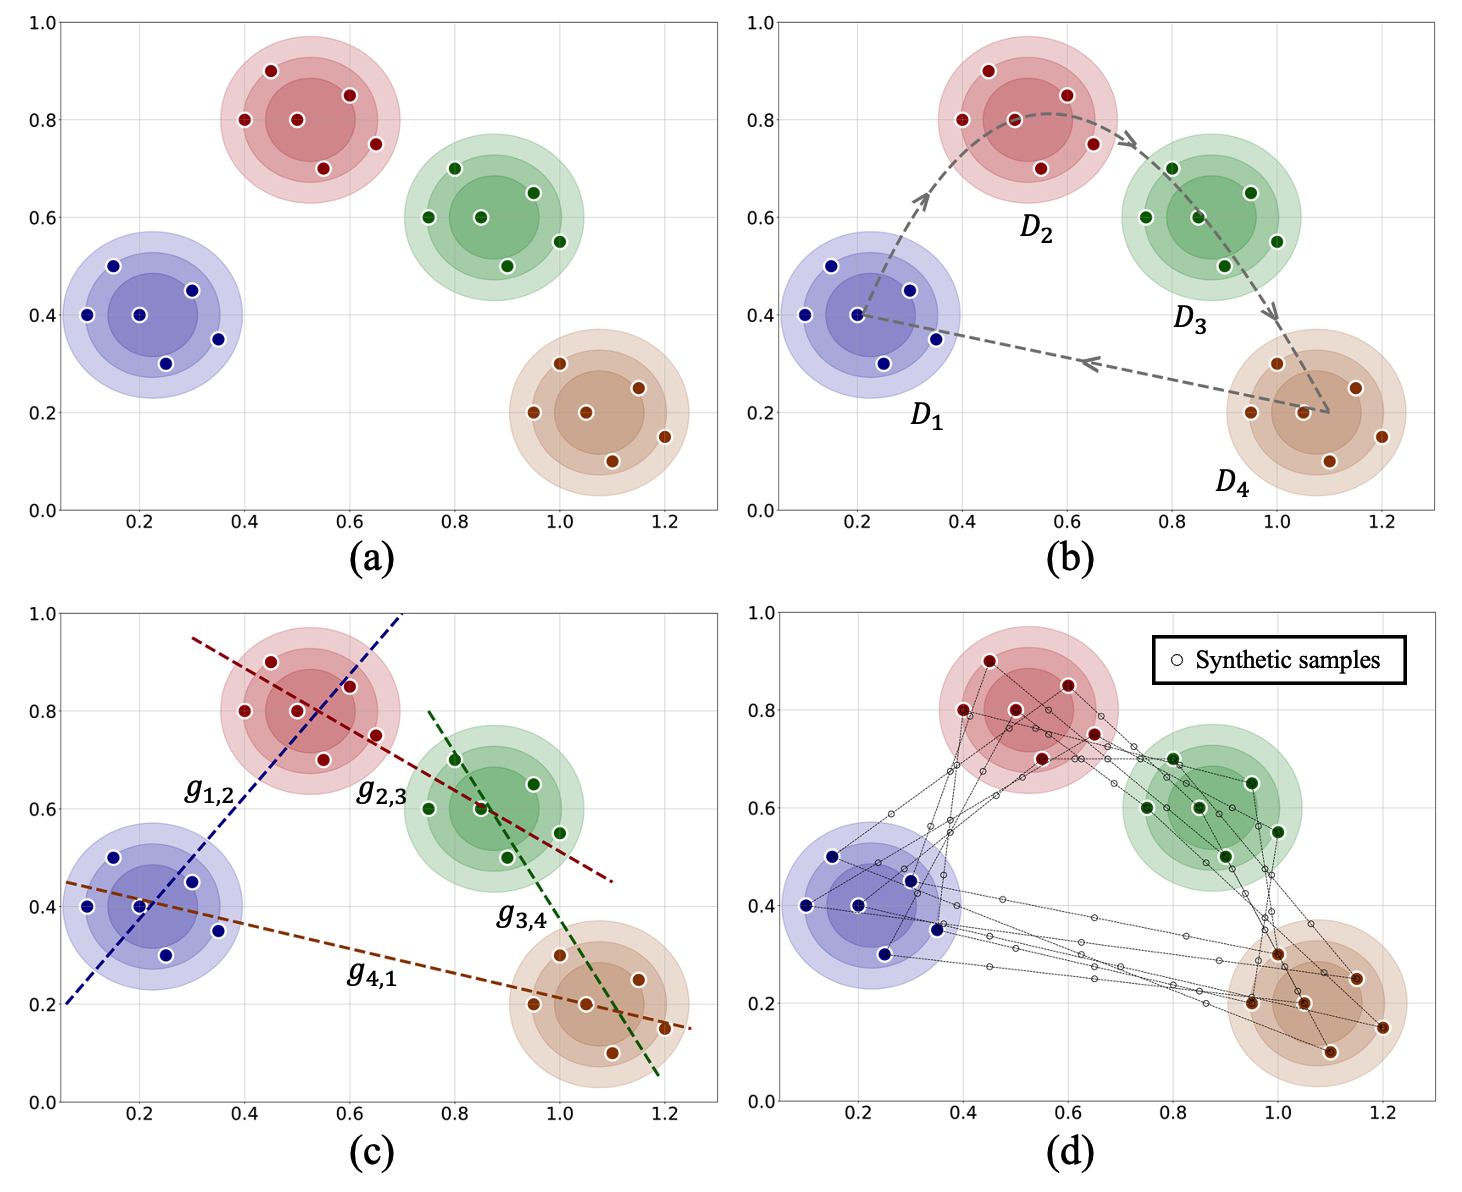
\includegraphics[scale=0.55]{Fig1.png}
  \caption{{The overall flowchart of the RSIS method in a 2D scenario.} (a) The 
  original feature space is divided into several feature 
  subspaces with approximately equal sample sizes through an 
  unsupervised clustering algorithm. (b) The TSP problem is 
  solved for the case of a two-dimensional feature space, 
  resulting in a subspace interpolation sorting scheme. (c) 
  Performing linear fitting between subspaces with adjacent 
  sorting. (d) Based on the results of linear fitting, four 
  sample interpolation matching strategies between adjacent 
  subspaces is obtained through the multi-stage minimum weight 
  matching method, and interpolation is performed to 
  synthesize samples with smaller errors.}
  \label{Fig1}
\end{figure*}

\subsection{Dividing of Feature Spaces}
We propose an unsupervised clustering algorithm that can 
partition the feature space into multiple subspaces with 
similar sample sizes. This algorithm consists of two stages: 
hierarchical clustering and the K-Nearest Neighbors 
optimization.

\subsubsection{Hierarchical Clustering}
The design of the hierarchical clustering process is 
primarily based on the concept of a greedy strategy, 
implemented through an unsupervised algorithm that 
aggregates clusters via multiple iterative cycles. 
An initial hyperparameter $k$ is required, where $k$ 
intuitively represents the number of subspaces into which 
the original feature space is partitioned. 

In the initial iteration process, an ordered set of sample 
features is given as $C_1=\left\{\boldsymbol{c}_i \right\}_{i=1}^n
=\left\{\boldsymbol{x}_i \right\}_{i=1}^n$, where the 
$\boldsymbol{c}_i$ is the $i\text{-th}$ element in set 
$C_1$. Subsequently, the closest pair of elements 
$\boldsymbol{c}_p$ and $\boldsymbol{c}_q$ within $C_1$ is 
identified, where $p,q=\mathop{\text{argmin}}_{\substack{p, q; p\neq {q}}} 
\text{dist}(\boldsymbol{c}_p,\boldsymbol{c}_q)$. Based on this, 
the set $D_{1}=\{\boldsymbol{c}_p,\boldsymbol{c}_q\}$, 
encompassing the two nearest elements, is defined as the first 
cluster, and calculate the centroid according to Formula \eqref{eq1}:
\begin{equation}
\label{eq1}
\bar{\boldsymbol{x}}^s = \frac{\sum_{\boldsymbol{x}^s \in D_s} 
\boldsymbol{x}^s}{\text{num}(D_s)}, 
\end{equation}
where $\text{num}(D_s)$ is the number of samples in set $D_s$. At 
the end of the first iteration, $\boldsymbol{c}_p$ and $\boldsymbol{c}_q$ are removed from the set $C_1$, and add the 
centroid of $D_1$ to $C_1$. i.e., $C_{2}=\{\boldsymbol{c}_i \in C_{1} | i \neq 
p, q\} \cup \{\bar{\boldsymbol{x}}^1\}$.

\begin{figure*}[t!]
  \centering
  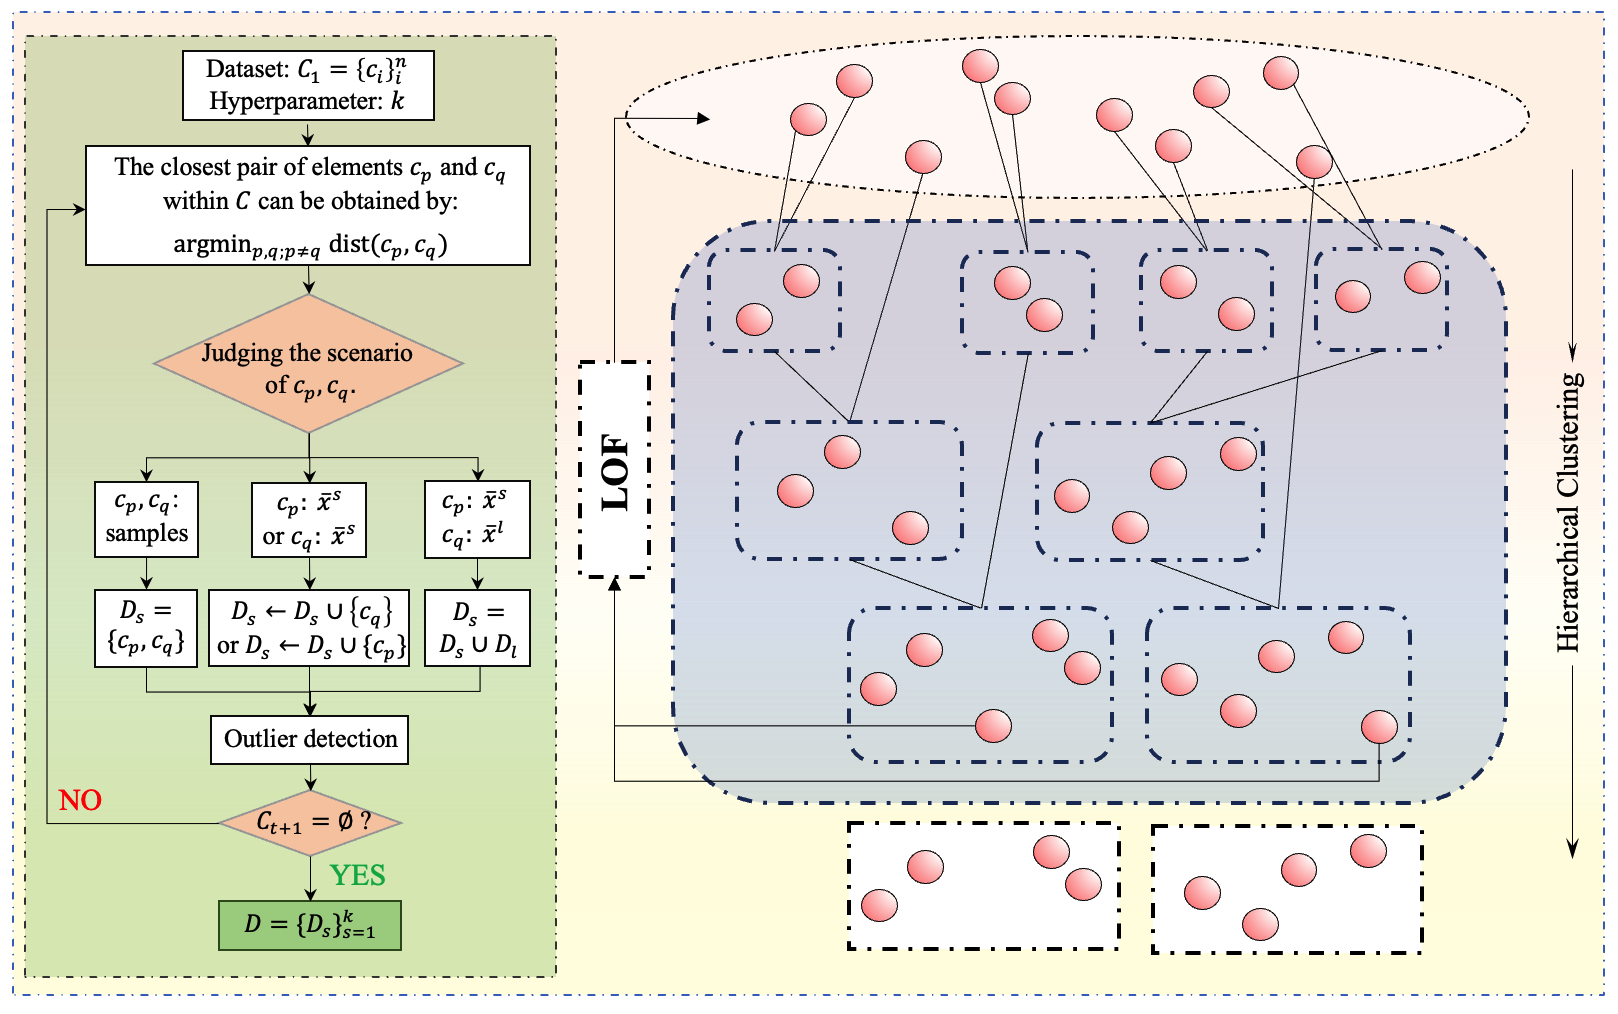
\includegraphics[scale=0.56]{Fig2.png}
  \caption{The hierarchical clustering process of RSIS.}
  \label{Fig2}
\end{figure*}

In subsequent iterations, it is required to determine the two 
elements $\boldsymbol{c}_p,\boldsymbol{c}_q$ with the closest 
distance in the set $C_t$. Three scenarios are considered 
for $\boldsymbol{c}_p$ and $\boldsymbol{c}_q$: both are 
original samples; one is a sample and the other is a cluster 
centroid; both are cluster centroids.

In the scenario where both $\boldsymbol{c}_p$ and $
\boldsymbol{c}_q$ are original samples, the set $D_s=\{
  \boldsymbol{c}_p,\boldsymbol{c}_q\}$ is defined as a new cluster 
  and its centroid $\bar{\boldsymbol{x}}^s$ is computed. 
  $\boldsymbol{c}_p$ and $\boldsymbol{c}_q$ are then removed 
  from set $C_t$ and $\bar{\boldsymbol{x}}^s$ is added to $C_t$, i.e.,
   $C_{t+1}=\{\boldsymbol{c}_i \in C_{t} | i \neq p, q\} \cup 
   \{\bar{\boldsymbol{x}}^s\}$.

In the scenario where $\boldsymbol{c}_p$ is an original sample and 
$\boldsymbol{c}_q:{\bar{\boldsymbol{x}}^s}$ is a cluster centroid, 
add $\boldsymbol{c}_p$ to $D_s$. Then, $\boldsymbol{c}_p$ is removed 
from set $C_t$, and the centroid of $D_s$ within $C_t$ is 
recalculated and updated according to Formula \eqref{eq1}, resulting in 
$C_{t+1}=\{\boldsymbol{c}_i \in C_{t} | i \neq p, q\}\cup \{ 
  \bar{\boldsymbol{x}}^{s^\prime} \}$.

If both $\boldsymbol{c}_p:{\bar{\boldsymbol{x}}^s}$ and $
\boldsymbol{c}_q:{\bar{\boldsymbol{x}}^l}$ are centroids, then 
the two clusters are merged by $D_s \leftarrow D_s  
{\cup}  D_l$, and the centroid of $D_s$ is recalculated. We can 
obtain $C_{t+1}=\{\boldsymbol{c}_i \in C_{t} | i \neq p, q\} \cup \{
  \bar{\boldsymbol{x}}^{s^\prime}\}$.

At the end of each iteration, if $\text{num}(D_s){\ge}\left\lceil 
n/k\right\rceil$, remove $\bar{\boldsymbol{x}}^s$ from $C_{t+1}$. 
Subsequently, the Local Outlier Factor (LOF) algorithm \cite{bib53} is 
employed to detect the outliers in $D_s$, and eliminate the 
superfluous samples $\{\boldsymbol{x}^s_i\}_{i=\left\lceil n/k
\right\rceil+1}^{\text{num}(D_s)}$ from $D_s$. $D_s$ is then 
considered a complete cluster and excluded from further iterations.
 Lastly, the redundant samples are 
 reinserted into $C_{t+1}$. The iterative process ends when 
$C_{t+1}=\emptyset$. The detailed procedural flow for this 
 segment can be referenced in Fig. \ref{Fig2}, and Algorithm \ref{Alg1}.

 \begin{algorithm}
  \caption{Hierarchical Clustering.}\label{alg:alg1}
  \begin{algorithmic}
  \STATE 
  \STATE $\mathbf{Input}$: the set of sample features $C$, hyperparameter $k$
  \STATE $\mathbf{Output}$: $D=\{D_s\}_{s=1}^k$
  \vspace{5pt} %在这里调整距离以达到期望的空间大小
  \STATE While: $C\neq\emptyset$:
  \STATE \hspace{0.5cm}Obtain $\boldsymbol{c}_p$ and $\boldsymbol{c}_q$ by $\mathop{\text{argmin}}_{\substack{p, q ; p \neq  {q}}}\text{dist}(\boldsymbol{c}_p,\boldsymbol{c}_q)$
  \STATE \hspace{0.5cm}Judging the situation of $\boldsymbol{c}_p$ and $\boldsymbol{c}_q$:
  \STATE \hspace{1.0cm}If both $\boldsymbol{c}_p$ and $\boldsymbol{c}_q$ are samples:
  \STATE \hspace{1.5cm}Define the new cluster $D_s=\{\boldsymbol{c}_p,\boldsymbol{c}_q\}$
  \STATE \hspace{1.5cm}Calculate the centroid of $D_s$ and add it to $C$
  \STATE \hspace{1.5cm}Remove $\boldsymbol{c}_p$ and $\boldsymbol{c}_q$ from $C$
  \STATE \hspace{1.0cm}Else if $\boldsymbol{c}_p:\bar{\boldsymbol{x}}^s$ or $\boldsymbol{c}_q:{\bar{\boldsymbol{x}}^s}$:
  \STATE \hspace{1.5cm}$D_s\leftarrow D_s {\cup} \{{\boldsymbol{c}}_q\}$ or $D_s\leftarrow D_s {\cup} \{{\boldsymbol{c}}_p\}$
  \STATE \hspace{1.5cm}Recalculate the centroid of $D_s$ and renew it in $C$
  \STATE \hspace{1.5cm}Remove $\boldsymbol{c}_q$ or $\boldsymbol{c}_p$ from $C$
  \STATE \hspace{1.0cm}Else if both $\boldsymbol{c}_p:{\bar{\boldsymbol{x}}^s}$ and $\boldsymbol{c}_q:{\bar{\boldsymbol{x}}^l}$ are centroids:
  \STATE \hspace{1.5cm}$D_s \leftarrow D_s  {\cup}  D_l$
  \STATE \hspace{1.5cm}Recalculate the centroid of $D_s$ and add it to $C$
  \STATE \hspace{1.5cm}Remove $\boldsymbol{c}_p$ and $\boldsymbol{c}_q$ from $C$
  \STATE \hspace{0.5cm}If $\text{num}(D_s)\ge \left\lceil n/k\right\rceil$:
  \STATE \hspace{1.0cm}Remove $\bar{\boldsymbol{x}}^s$ from $C$
  \STATE \hspace{1.0cm}Detect the redundant samples in $D_s$ by LOF algorithm
  \STATE \hspace{1.0cm}Remove $\{\boldsymbol{x}^s_i\}_{i=\left\lceil n/k\right\rceil+1}^{\text{num}(D_s)}$ from $D_s$ and add them to $C$
  \STATE \hspace{1.0cm}$D \leftarrow D  {\cup}  D_s$
  \end{algorithmic}
  \label{Alg1}
\end{algorithm}

Consequently, the iterative process can partition the original 
dataset into $k-1$ subsets, each containing an equal number 
of samples; and one additional subset consisting of no more 
than $\left\lceil n/k\right\rceil$ samples. Formally, we 
define $D={\cup}^k_{s=1}D_s$, $D_s=\{\boldsymbol{x}_i\}_{i=1}^l$, 
where $1 {\le} l {\le} \left\lceil n/k\right\rceil$. Moreover, the 
iterative clustering process of RSIS results in the division of 
the original feature space into $k$ feature subspaces, represented 
as $\mathcal{X} = \cup_{s=1}^{k} \mathcal{X}^s$.

During the iterative hierarchical clustering process, it is 
required to identify the two closest elements in $C_t$. This step 
can be optimized using the K-dimensional tree (K-d tree) method. 
The construction of a K-d tree typically has a time complexity 
of $O(n\log{n})$, and the average time complexity for deleting or 
adding a point and finding the two nearest elements in a K-d 
tree is $O(\log{n})$. However, as the iteration proceeds, the 
sample size gradually decreases, hence the actual search time 
will slightly decline. Excluding the LOF algorithm which may 
reassign redundant samples from a cluster back to the dataset, 
the total number of iterations is $n$. If the K-d tree is not 
rebuilt at every iteration, and the operations of querying and 
updating are efficient on an existing K-d tree, the overall 
time complexity might indeed be closer to $O(n\log{n})$.





\subsubsection{K-Nearest Neighbors Optimization}
The hierarchical clustering process, being based on the concept 
of a greedy strategy, may yield irrational outcomes in later 
iterations, which affects the overall clustering performance. 
Consequently, an optimization process utilizing K-Nearest 
Neighbors (KNN) has been developed to fine-tune the clustering 
results. This approach may affect the balance of the number of 
samples in each cluster, but it will significantly improve the 
performance of the clustering.

\begin{figure}[t!]
  \centering
  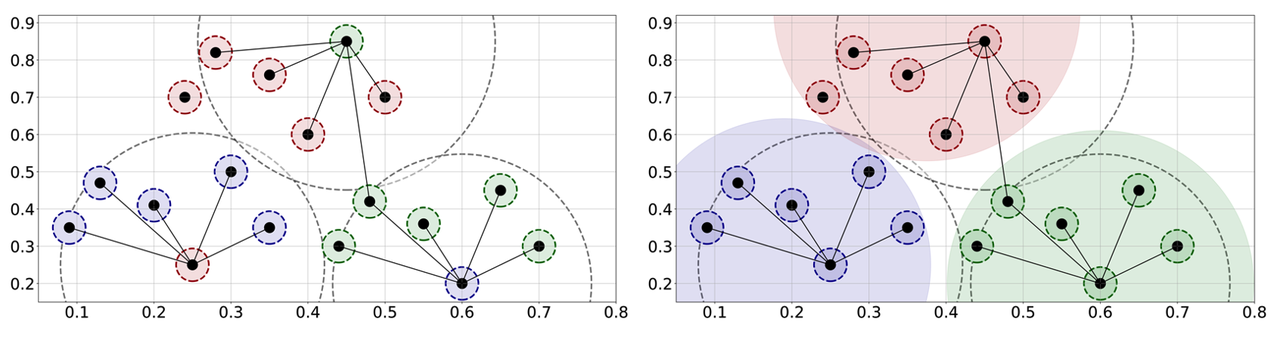
\includegraphics[scale=0.3]{Fig3.png}
  \caption{K-Nearest Neighbors optimization.}
  \label{Fig3}
\end{figure}

Upon completing the hierarchical clustering phase, each sample 
is endowed with a label reflecting its cluster membership. 
During the KNN optimization phase, the algorithm identifies 
the $\left\lceil n/k\right\rceil$ nearest neighbors for each 
sample in the feature space. Each sample's cluster label is then 
updated to reflect the most frequently occurring cluster label 
among its neighbors. It is important to note that this process 
may induce changes in the cluster affiliation of some samples, 
thereby causing slight fluctuations in the number of samples 
within clusters. Such alterations could result in the dissolution 
of clusters with a more dispersed sample distribution. By 
integrating the hierarchical clustering process with KNN 
optimization, we arrive at the final clustering results 
$\{D_s\}_{s=1}^{k'}$, where $k'$ denotes the number of clusters 
post-optimization. This algorithmic approach, depicted in 
Fig. \ref{Fig3}, ensures the uniform distribution of sample sizes 
across clusters, significantly enhancing the overall performance 
of clustering.





\subsection{Subspace Interpolation Path Sorting}
The design philosophy of the interpolation path involves starting 
from a subspace, traversing each subspace exactly once, and 
ultimately returning to the original point. 
{The aim is to minimize the total distance of the path between centroids of clusters (subspaces).} 
This challenge can be formulated 
as TSP, which is then addressed 
by depicting the issue as a weighted graph. Bridging this concept 
to our ultimate goal, the objective function is defined as:
\begin{equation}
\label{eq2}
\min{\sum\limits_{i=1}^{k'-1}\text{dist}(\boldsymbol{\bar{x}}^i,
\boldsymbol{\bar{x}}^{i+1})}+\text{dist}(\boldsymbol{\bar{x}}^{k'},
\boldsymbol{\bar{x}}^1). 
\end{equation}

The TSP is a classic NP-hard problem 
in combinatorial optimization, posing significant challenges in 
finding polynomial-time solutions as graph complexity increases. 
Widely applicable in logistics, planning, and manufacturing, 
the TSP's direct solution is complex, prompting the development 
of heuristic and approximation algorithms to seek near-optimal 
solutions efficiently \cite{bib56,bib57}. To ensure that a sufficiently good 
solution can be obtained within an acceptable timeframe, we first 
employ a greedy algorithm to quickly find an initial solution, 
which is then optimized using the 3-opt method to arrive at the 
final solution \cite{bib61,bib64}, as is shown 
in Fig. \ref{Fig4}. Ultimately, a sorted set 
$D_\text{sorted}=\{D_{(s)}\}_{s=1}^{k'}$ is obtained. Corresponydingly, $\mathcal{X}_{\text{sorted}}=\cup_{s=1}^{k^\prime}\mathcal{X}^{(s)}$. In the subsequent sections of this paper, the feature 
subspace corresponding to two subsets with adjacent indices will be 
defined as adjacent feature subspaces.

\begin{figure}[h!]
  \centering
  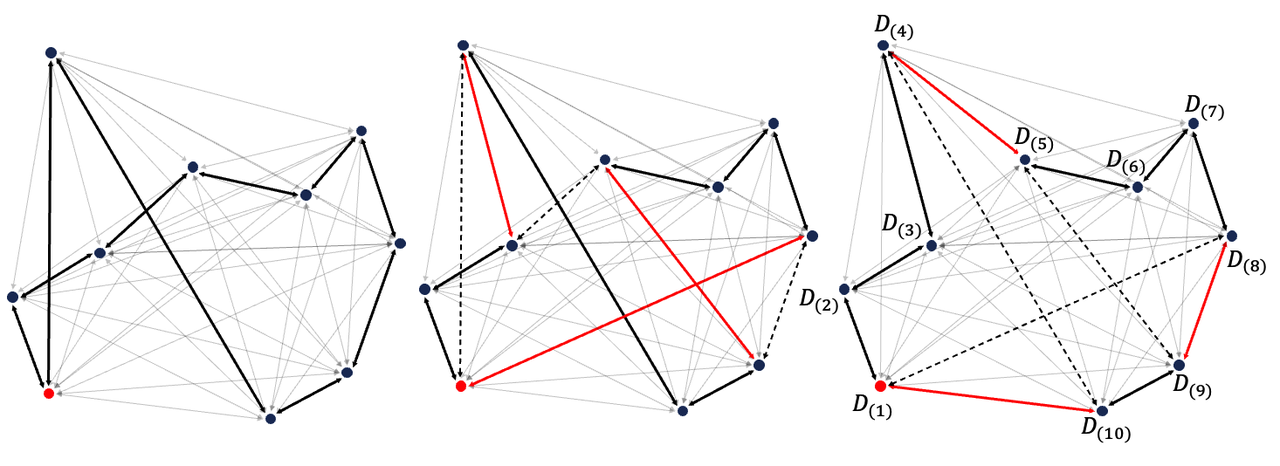
\includegraphics[scale=0.3]{Fig4.png}
  \caption{Greedy algorithm and 3-opt solved for TSP in 
  two-dimensional feature space.}
  \label{Fig4}
\end{figure}

The above discussion applies to multidimensional feature spaces. 
However, in the case of a one-dimensional feature space, given 
the unique characteristics of one-dimensional spaces, the design 
of the interpolation path still requires passing through all 
subspaces exactly once, but it does not necessitate returning to 
the starting point. A greedy strategy can be directly employed to 
solve this, and in the one-dimensional case, the solution obtained 
by this method is guaranteed to be optimal. First, the starting 
subspace of the interpolation path is identified:
\begin{equation}
\label{eq3}
D_{(1)}=\mathop{\text{argmin}}_{\substack{D_{(s)}\in D_{\text{sorted}}}}
\text{dist}({\bar{x}}^s,{x}_0), 
\end{equation}
where $x_0$ is the minimum value in feature set. The definition 
for subsequent clusters is as follows:
\begin{equation}
\label{eq4}
D_{(d)} = \mathop{\text{argmin}}_{\substack{D_{(s)} \in D_{\text{sorted}}; \\ 
D_{(s)} \neq D_{(1)}, \ldots, D_{(d-1)}}}\text{dist}\left(\bar{x}^s, 
\bar{x}^{s-1}\right).
\end{equation}

Unless otherwise specified, the subsequent research in this paper 
will primarily focus on exploring the case of multidimensional 
feature spaces.

\subsection{Adjacent Subspace Linear Regression Fitting}
Given a dataset with noise $D=\{\boldsymbol{x}_i,y_i\}_{i=1}^n$, 
where $\boldsymbol{x}_i\in \mathcal{X}=\mathbb{R}^d$ and 
$y_i\in\mathcal{Y}=\mathbb{R}$. Assume that 
$\dot{y}_i=f(\dot{\boldsymbol{x}}_i)$, where 
$\dot{\boldsymbol{x}}_i$ represents the denoised true value of 
$\boldsymbol{x}_i$, and $\dot{y}_i$ is the true value of 
$y_i$. The RIRS method presupposes that the function $f(\cdot)$ 
is continuous. And we have:
\begin{align} 
\label{eq5}
\dot{y}_i+\varepsilon_{i,y}=f(\dot{\boldsymbol{x}}_i+
\boldsymbol{\varepsilon}_{i,x})+\varepsilon_i, 
\end{align}
where $\boldsymbol{\varepsilon}_{ix}$ and $\varepsilon_{i,y}$ 
respectively represent the noise contained in 
$\dot{\boldsymbol{x}}_i$ and $\dot{y}_i$, $\varepsilon_i$ is the 
error term of the equation. Equation \eqref{eq5} can be transformed into:
\begin{equation} 
\label{eq6}
y_i=f(\boldsymbol{x}_i)+\varepsilon_i. 
\end{equation}

Through the aforementioned clustering and subspace sorting 
algorithms, the dataset $D$ can be partitioned into multiple 
ordered subsets $D_{\text{sorted}}=\{D_{(s)}\}_{s=1}^{k^\prime}$, 
where $D_{(s)}=\{ \boldsymbol{x}_i^s,y_i^s \}_{i=1}^{\text{num}
(D_{(s)})}$, and the feature space can be divided into multiple 
subspaces $\mathcal{X}_{\text{sorted}}=\cup_{s=1}^{k^\prime}\mathcal{X}^{(s)}$. For 
two adjacent feature subspaces, given that the RSIS method assumes 
the relation $f(\cdot)$ to be a continuous function, it allows 
$f(\cdot)$ to be approximately fitted as a linear function 
$g(\cdot)$, hence Equation \eqref{eq6} can be transformed into: 
\begin{equation} 
\label{eq7}
y_i^{s,s+1}=g_{s,s+1}(\boldsymbol{x}_i^{s,s+1})+\varepsilon_i+
\varepsilon_i^\prime, 
\end{equation}
where $g_{s,s+1}(\cdot)$ and $\varepsilon_i^\prime$ respectively 
denote the linear fitting function between adjacent feature 
subspaces $\mathcal{X}^{(s)}$ and $\mathcal{X}^{(s+1)}$, and the linear 
fitting error, $\{\boldsymbol{x}_i^{s,s+1},y_i^{s,s+1}\}\in D_{(s)}\cup 
D_{(s+1)}$. If the distance between two subspaces is sufficiently 
close and the measure of the subspaces tends towards $0$, then the 
linear fitting error $\varepsilon_i^\prime\rightarrow0$.

One may consider employing methods such as Ordinary Least Squares 
(OLS), Lasso regression, or locally weighted linear regression to 
estimate $g_{s,s+1}(\cdot)$. 
However, given the assumption that $f(\cdot)$ is a continuous 
function, merely conducting linear fitting based on samples from 
two subspaces does not adequately take into account global 
information. Therefore, we integrate the principle of soft 
parameter sharing mechanisms \cite{bib70,bib71}, estimating linear functions 
among multiple subspaces simultaneously, and incorporates the number of $k^\prime$ 
$L_1$ regularization term in the design of the loss function. This approach ensures that the estimation of each linear function 
$\hat{g}_{s,s+1}(\cdot)$ incorporates global information to the 
greatest extent possible:
\begin{equation} 
\label{eq8}
\begin{aligned}
L(\boldsymbol{\beta})=
&\sum\limits_{s=2}^{k^\prime-1}
\left(L_2(\boldsymbol{\beta}^{s,s+1})+\dfrac{\lambda}
{\text{dist}(\overline{\boldsymbol{x}}^{s},
\overline{\boldsymbol{x}}^{s-1})+1} 
L_1(\boldsymbol
{\beta}^{s,s+1},\boldsymbol{\beta}^{s-1,s}) \right) 
+L_2(\boldsymbol{\beta}^{1,2})+L_2(\boldsymbol{\beta}
^{k^\prime,1}) \\
&\quad+\dfrac{\lambda}{\text{dist}(
  \overline{\boldsymbol{x}}^{k^\prime},\overline
  {\boldsymbol{x}}^{k^\prime-1})+1}L_1(\boldsymbol{\beta}^{k^\prime,1},
  \boldsymbol{\beta}^{k^\prime-1,k^\prime})+\dfrac{\lambda}{\text{dist}(
\overline{\boldsymbol{x}}^{k^\prime},\overline
{\boldsymbol{x}}^{1})+1}L_1(\boldsymbol{\beta}^{1,2},
\boldsymbol{\beta}^{k^\prime,1}), 
\end{aligned}
\end{equation}
where $\boldsymbol{\beta}=\left(\boldsymbol{\beta}
^{1,2},\boldsymbol{\beta}^{2,3},\ldots,\boldsymbol
{\beta}^{k^\prime-1,k^\prime},\boldsymbol{\beta}^
{k^\prime,1}\right)^\prime$, $L_2(\boldsymbol{\beta}
^{p,q})=\left\|\boldsymbol{y}^{p, q}-\boldsymbol{X}^{p, q} 
\boldsymbol{\beta}^{p, q}\right\|_{2}^{2}$, 
$L_1(\boldsymbol{\beta}^{q,r},\boldsymbol{\beta}^
{p,q})=\|\boldsymbol{\beta}^{q,r}-\boldsymbol{\beta}
^{p,q}\|_1$ and $\dfrac{\lambda}{\text{dist}(
\overline{\boldsymbol{x}}^{s},\overline{\boldsymbol{x}}
^{s-1})+1}$ serves as the coefficient for the 
regularization term, adaptively adjusted based on 
the distance between subspaces. In the subsequent 
simulation experiments and case analyses, $\lambda$ 
is set to $1$.

Theorem \ref{the1}, presented later, builds directly upon the 
foundational results established by Lemma \ref{lem1} and 
Lemma \ref{lem2}. By proving the convexity of the loss 
function through Theorem \ref{the1}, we ensure the attainment 
of the global minimum and facilitate the application 
of optimization algorithms with guaranteed convergence 
properties. Detailed proofs are provided in the 
Appendix.

\begin{lemma}
\label{lem1}
For the function $f(\boldsymbol{\beta})=\|\boldsymbol{y}-
\boldsymbol{X}\boldsymbol{\beta}\|_2^2$, where 
$\boldsymbol{y}\in\mathbb{R}^{n\times1}$, $\boldsymbol{X}\in
\mathbb{R}^{n\times d}$, and $\boldsymbol{\beta}\in\mathbb{R}
^{d\times1}$. For $\forall\omega\in[0,1]$, and $\forall\boldsymbol
{\beta}_1,\boldsymbol{\beta}_2\in\mathbb{R}^{d\times1}$, it can 
be obtained:
\begin{equation}
\label{eq9}
f(\omega\boldsymbol{\beta}_1+(1-\omega)\boldsymbol{\beta}_2)
\le\omega f(\boldsymbol{\beta}_1)+(1-\omega)f(\boldsymbol{\beta}_2).
\end{equation}
\end{lemma}

\begin{lemma}
\label{lem2}
For the function $f(\boldsymbol{\beta})=\|\boldsymbol{\beta}^1-
\boldsymbol{\beta}^2\|_1$, where $\boldsymbol{\beta}^1,\boldsymbol
{\beta}^2\in\mathbb{R}^{d\times1}$, $\boldsymbol{\beta}=(
(\boldsymbol{\beta}^1)^\prime,(\boldsymbol{\beta}^2)^\prime)
^\prime$. For $\forall\omega\in[0,1]$, and $\forall\boldsymbol
{\beta}_1,\boldsymbol{\beta}_2\in\mathbb{R}^{2d\times1}$, one 
can infer:
\begin{equation}
\label{eq10}
f(\omega\boldsymbol{\beta}_1+(1-\omega)\boldsymbol{\beta}_2)\le
\omega f(\boldsymbol{\beta}_1)+(1-\omega)f(\boldsymbol{\beta}_2).
\end{equation}
\end{lemma}

\begin{theorem}
\label{the1}
For the Equation \eqref{eq8}, $\forall\omega\in[0,1]$, 
and $\forall\boldsymbol{\beta}_1,\boldsymbol{\beta}_2\in
\mathbb{R}^{d\times k^\prime}$, it can be derived:
\begin{equation}
\label{eq11}
L(\omega\boldsymbol{\beta}_1+(1-\omega)\boldsymbol{\beta}_2)
\le\omega L(\boldsymbol{\beta}_1)+(1-\omega)L(\boldsymbol{\beta}_2).
\end{equation}
\end{theorem}

\subsection{Multi-Stage Minimum Weight Matching}
In the subsequent steps, we will synthesize new samples by 
performing linear and equidistant interpolation between adjacent 
subspaces. The samples synthesized by the RSIS take into account 
all sample information comprehensively, and the interpolation 
rules are designed as follows:

\begin{itemize}
  \item The two samples used for linear interpolation should 
  originate from distinct and adjacent subspaces.
  \item Each sample must participate in the interpolation 
  process at least once.
  \item The interpolation will be performed a total of 
  $\max(\text{num}{(D_{(s)}),\text{num}(D_{(s+1)})})$ times.
  \item The participation frequency in interpolation for all 
  samples must be uniform. Specifically, each sample is allowed 
  to participate in the interpolation process up to 
  $\left\lceil \frac{\max(\text{num}{(D_{(s)}),
  \text{num}(D_{(s+1)})})}{\min(\text{num}{(D_{(s)}),
  \text{num}(D_{(s+1)})})}\right\rceil$ times.
\end{itemize}

Without loss of generality, we 
assume that $\text{num}(D_{(s)})=m$, $\text{num}(D_{(s+1)})=n$, 
and $n/2\le m \le n$. According to the rules of interpolation, 
there are $C_{n-2k}^{2}\prod_{k=0}^{n-m-1} C_{m}^{n-m}(2m-n)!$ 
interpolation matching strategies available for selection. 
Seeking a suboptimal matching strategy is a crucial problem 
that we need to tackle.

Similarly, without loss of generality, assuming that the feature 
space is one-dimensional. The average error of samples synthesized 
through linear and equidistant interpolation between two original 
samples is measured by:
\begin{equation} 
\label{eq12}
\bar{S}(x^s,x^{s+1})=\frac{\int_{x^s}^{x^{s+1}}|f(x)-l(x)|  dx}
{|x^{s+1}-x^s|}, 
\end{equation}
where $l(x)$ denotes the linear function passing through points 
$(x^s,y^s)$ and $(x^{s+1},y^{s+1})$, and $f(\cdot)$ represents
 the real function of $x$ and $y$. 

\begin{theorem}
\label{the2}
For two adjacent subspaces $\mathcal{X}^{(s)}$ and $\mathcal{X}^{(s+1)}$, 
consider $(x^s,y^s)\in D_{(s)}\;\text{and}\; (x^{s+1},y^{s+1})
\in D_{(s+1)}$, with $y=f(x)+\varepsilon$. According to \eqref{eq7}, 
assuming the linear fitting error $\varepsilon^\prime\rightarrow0$. 
It can be obtained that:c
\begin{equation}
\label{eq13}
\mathbb{E} (\bar{S}(x^s,x^{s+1}))< \mathbb{E}(\frac{|\varepsilon^s|
+|\varepsilon^{s+1}|}{2}).
\end{equation}
\end{theorem}

From Theorem 2, under the assumption of the linear fitting error 
$\varepsilon_i^\prime\rightarrow0$, linear interpolation between 
samples from any two adjacent subspaces will result in a lower expected 
average error for the interpolated synthetic samples compared to 
the {original}   samples, even in the scenario where noise with different 
distributions. 

\begin{theorem}
\label{the3}
Extending the groundwork established in Theorem 2, let 
$y^s=f(x^s)+\varepsilon^s$, $y^{s+1}=f(x^{s+1})+\varepsilon^{s+1}$.
 Assuming the linear fitting error $\varepsilon^\prime
 \rightarrow0$. We have: 
\begin{equation}
\label{eq14}
\begin{aligned}
\bar{S}(x^s,x^{s+1})
=
\begin{cases} 
\dfrac{|\frac{\varepsilon^s}{\varepsilon^s-\varepsilon^{s+1}}|
\cdot |\varepsilon^{s}|+|\frac{\varepsilon^{s+1}}{\varepsilon^s-
\varepsilon^{s+1}}|\cdot|\varepsilon^{s+1}|}{2},\quad\varepsilon^s
\cdot \varepsilon^{s+1}<0,
\\
\dfrac{|\varepsilon^s|+|\varepsilon^{s+1}|}{2}, 
\;\qquad\qquad\qquad\qquad\varepsilon^s\cdot 
\varepsilon^{s+1}\ge0.
\end{cases}
\end{aligned}
\end{equation}
\end{theorem}


According to Theorem 3, Formula \eqref{eq12} can be transformed into 
Formula \eqref{eq14}. We can first estimate the error of the samples, 
and then determine the matching strategy based on the error 
information by employing the method of bipartite graph minimum 
weight matching. The noise of the samples can be estimated by the 
linear fitting function between adjacent subspaces, under the 
assumption conditions, as can be derived from Equation \eqref{eq7}:
\begin{equation} 
\label{eq15}
\varepsilon_i^{s,s+1}=y_i^{s,s+1}-g_{s,s+1}(\boldsymbol{x}_i^
{s,s+1}).
\end{equation} 

According to interpolation rules, each sample is mandated to 
undergo at least one interpolation, and the total number of 
interpolations is constrained. After optimization with the KNN, 
the number of samples between subspaces is not always exactly 
equal, thus this cannot be considered a classical minimum weight perfect 
matching problem. This problem represents a variant of the 
weighted matching problem, incorporating features of both 
balanced matching and minimum weight matching, as it necessitates 
minimizing the total weight of matching while also ensuring the 
uniformity of sample matching occurrences. Currently, there is 
no standard algorithm readily available for this specific 
problem, necessitating modifications to the traditional minimum 
weight matching approach to accommodate this target scenario. 
Based on this, we propose a heuristic multi-stage minimum weight 
matching algorithm. Note that this method does not guarantee an 
optimal solution, but it can obtain a reasonable suboptimal 
solution in a short time.

Continuing with the previous assumption $\text{num}(D_{(s)})=m$, $\text{num}(D_{(s+1)})=n$, $n/2\le m\le n$. In this scenario, each 
sample in $D_{(s)}$ is considered for either one or two
 matches, and the solution is approached in two stages. Given a 
 weighted bipartite graph $G=(D_{(s)},D_{(s+1)},E)$ with a weight 
 function $\omega:E\rightarrow\mathbb{R}$, where $D_{(s)}$, $D_{(s+1)}$ 
 are the sets of vertices on the two sides and $E\subseteq D_{(s)}
 \times D_{(s+1)}$ is the set of edges. According to Formula 
 \eqref{eq14}, let the weight function $\omega(\boldsymbol{x}^{s},
 \boldsymbol{x}^{s+1})=\bar{S}(\boldsymbol{x}^{s},\boldsymbol{x}
 ^{s+1})$. Consider the objective function:
\begin{equation*}
\begin{aligned}
&\text{min}\textstyle\sum\limits_{(i,j)\in{E}}\omega(\boldsymbol{x}^{s}_i,\boldsymbol{x}_j^{s+1})v_{i,j},\\
&s.t. \;\;
\textstyle\sum\limits_{j=1}^nv_{i,j} \in\{1,2\}\;\text{for}\;\forall i, \\
&\quad\;\;\;\textstyle\sum\limits_{i=1}^mv_{i,j} =1\;\text{for}\;\forall j,
\end{aligned}
\end{equation*}
where $v_{i,j}$ is a binary decision variable. In the first stage, 
without considering any constraints, the Hungarian algorithm is 
applied directly to the bipartite graph $G$ to obtain a solution, 
resulting in a maximum matching $M_1$ for $G$. At this point, 
each vertex $\boldsymbol{x}^s\in D_{(s)}$ is matched once, $m$ 
vertices from $D_{(s+1)}$ are also matched once, and the 
remaining $n-m$ vertices in $D_{(s+1)}$ remain unmatched, which 
are denoted as $D^\prime_{(s+1)}$.

In the second stage, define $G'=(D_{(s)},D'_{(s+1)},E')$ with 
$\omega$, where $E'\subseteq D_{(s)}\times D'_{(s+1)}$. Still 
employing the Hungarian algorithm for $G'$ to obtain $M_2$. Since 
$n/2\le m\le n$, each vertex in $D'_{(s+1)}$ is involved in one 
matching in $M_2$ and $n-m$ vertices from $D_{(s)}$ participate 
in a matching again. The final matching is obtained $M=M_1\cup
{M_2}$.



The above describes a two-stage minimum weight matching method 
for a specific assumed situation, which is also the most common 
scenario in sample matching between subspaces. If there is a 
significant difference in the number of samples between the two 
subspaces, the problem needs to be divided into 
$\left\lceil \frac{\max(\text{num}{(D_{(s)}),\text{num}
(D_{(s+1)})})}{\min(\text{num}{(D_{(s)}),\text{num}(D_{(s+1)})})}
\right\rceil$ stages for resolution, with a more general form presented in Algorithm \ref{Alg2}.

{The computational complexity of our proposed multi-stage minimum weight matching algorithm is analyzed as follows. Given a bipartite graph with $m$ vertices on one side and $n$ vertices on the other side $(m < n)$, the algorithm performs $\lceil n / m \rceil$ stages of minimum weight matching. Each stage uses the Hungarian algorithm, which has a time complexity of $O(m^2 \cdot n)$. Therefore, the overall computational complexity of the multi-stage matching process is $O(\lceil n / m \rceil \cdot m^2 \cdot n)$, which simplifies to $O(n^2 \cdot m)$.}

\begin{algorithm}[t!]
  \caption{Multi-Stage Minimum Weight Matching.}\label{alg:alg2}
  \begin{algorithmic}
  \STATE 
  \STATE $\mathbf{Input}$: $D_{(s)}=\{\boldsymbol{x}_i^{s},y_i^s\}_{i=1}^m$, $D_{(s+1)}=\{\boldsymbol{x}_i^{s+1},y_i^{s+1}\}_{i=1}^n\;(n\ge m)$, $\hat{g}_{s,s+1}$
  \STATE $\mathbf{Output}$: Interpolation matching strategy $M$
  \vspace{5pt} %在这里调整距离以达到期望的空间大小
  \STATE Estimate the error of $D_{(s)}$ and $D_{(s+1)}$ by {$\varepsilon_i^{s,s+1}=y_i^{s,s+1}-g_{s,s+1}(\boldsymbol{x}_i^
  {s,s+1})$}
  \STATE Define $G_1=(D_{(s)},D_{(s+1)},E)$ with $\omega(\boldsymbol{x}^{s},\boldsymbol{x}^{s+1})=\bar{S}(\boldsymbol{x}^{s},\boldsymbol{x}^{s+1})$
  \STATE For $t=1,2,\ldots,\left\lceil\frac{n}{m}\right\rceil$ do:
  \STATE \hspace{0.5cm}Utilizing the Hungarian algorithm on bipartite graph $G_t$ to obtain a maximum matching $M_t$
  \STATE \hspace{0.5cm}{$M\leftarrow{M}\cup{M_t}$
  \STATE \hspace{0.5cm}Define $D_{\text{matched}}\subset{D_{(s+1)}}$ which have been matched in $M_t$
  \STATE \hspace{0.5cm}$D^\prime_{(s+1)}\leftarrow D_{(s+1)}-D_{\text{matched}}$
 
  \STATE \hspace{0.5cm}Define $G_{t+1}=(D_{(s)},D'_{(s+1)},E')$, where $E'\subseteq D_{(s)}\times D'_{(s+1)}$}

  \end{algorithmic}
  \label{Alg2}
\end{algorithm}


\subsection{RSIS Overall Analysis}
Given that the number of subspaces is $k^\prime$, it is necessary 
to perform $k^\prime$ times of multi-stage minimum weight matching 
to obtain $k^\prime$ matching strategies, ultimately yielding 
the total distance of interpolation paths between all samples, 
denoted as $\text{dist}_{\text{sum}}$. An additional 
hyperparameter $\eta$ must be specified, which intuitively 
represents the ratio of the number of synthetic samples to the 
original sample size. For two samples from adjacent subspaces, 
$\{\boldsymbol{x}^s,y^s\}$ and $\{\boldsymbol{x}^{s+1},y^{s+1}\}$, 
the synthesized samples are given by $\{\boldsymbol{x}_{(d)}^
{s,s+1},y_{(d)}^{s,s+1} \}_{d=1}^{\left\lceil \frac{n\eta }
{\text{dist}_{\text{sum}}}\text{dist}(\boldsymbol{x}^s,
\boldsymbol{x}^{s+1})\right\rceil}$, where $n$ is the original 
sample size, and the term $\frac{n\eta}{\text{dist}_{\text{sum}}}$
 is intuitively the number of samples inserted per unit distance, 
 while $\left\lceil \frac{n\eta}{\text{dist}_{\text{sum}}}
 \text{dist}(\boldsymbol{x}^s,\boldsymbol{x}^{s+1})\right\rceil$ 
 is the total number of inserted samples between two original 
 samples. Assuming all variables are continuous, 
 the linear interpolation formula is designed as follows:
\begin{equation}
\label{eq16}
\boldsymbol{x}^{s,s+1}_{(d)}=\boldsymbol{x}^s+d\dfrac
{\boldsymbol{x}^{s+1}-\boldsymbol{x}^{s}}{\left\lceil 
\frac{n\eta}{\text{dist}_{\text{sum}}}\text{dist}
(\boldsymbol{x}^s,\boldsymbol{x}^{s+1})\right\rceil+1},
\end{equation}

\begin{equation}
\label{eq17}
y^{s,s+1}_{(d)}=y^s+d\dfrac{y^{s+1}-y^{s}}{\left\lceil 
\frac{n\eta}{\text{dist}_{\text{sum}}}\text{dist}
(\boldsymbol{x}^s,\boldsymbol{x}^{s+1})\right\rceil+1}.
\end{equation}



This approach allows for the adaptive control of the quantity of 
generated samples based on the distance between samples in the 
feature space, ensuring that inserted samples are linear and 
equidistant. Theorems \ref{the2} and \ref{the3} 
have essentially proved the effectiveness of the RSIS method. 
To ensure thoroughness and academic rigor, we additionally 
present a proof in Theorem \ref{the4} adhering to the interpolation 
format specified in Equations \eqref{eq16} and \eqref{eq17}. This method is delineated into multiple steps, with the overall 
operational procedure presented in Algorithm \ref{Alg3}.

\begin{algorithm}[h!]
  \caption{RSIS Method.}\label{alg:alg3}
  \begin{algorithmic}
  \STATE 
  \STATE $\mathbf{Input}$: Dataset $D=\{\boldsymbol{x}_i,y_i \}_{i=1}^n$,
  Hyperparameters $k,\eta$
  \STATE $\mathbf{Output}$: Synthesized dataset $D^\prime$
  \vspace{5pt} %在这里调整距离以达到期望的空间大小
  \STATE Construct feature dataset: $C=\{\boldsymbol{x}_i\}_{i=1}^n$
  \STATE Apply the hierarchical clustering algorithm to samples to obtain clusters $D=\{D_s\}_{s=1}^{k}$
  \STATE After KNN optimization, obtain: $D=\{D_s\}_{s=1}^{k^\prime}$
  \STATE Utilize greedy algorithm and 3-opt to obtain the sorted solution: $D_{\text{sorted}}=\{D_{(s)}\}_{s=1}^{k^\prime}$
  \STATE Perform linear fitting between adjacent subspaces to derive $\{\hat{g}_{s,s+1}\}_{s=1}^{k^\prime-1}\cup\{\hat{g}_{k^\prime,1}\}$
  \STATE For $s=1,2,\ldots,k^\prime$ do:
  {\STATE \hspace{0.5cm}$D_{(s+1)}=D_{(1)}$ if $s=k^\prime$}
  \STATE \hspace{0.5cm}Estimate the error in adjacent subspaces samples from $D_{(s)},D_{(s+1)}$ by \eqref{eq15}
  \STATE \hspace{0.5cm}Employ the multi-stage minimum weight matching method to determine the interpolation matching strategy
  \STATE \hspace{0.5cm}According to the matching strategy, interpolate between adjacent subspaces samples to synthesize 
new data
  \STATE \hspace{0.5cm}Add the newly synthesized data to $D^\prime$
  \end{algorithmic}
  \label{Alg3}
\end{algorithm}

\begin{theorem}
\label{the4}
For two adjacent subspaces $\mathcal{X}^{(s)}$ and 
$\mathcal{X}^{(s+1)}$, consider $(\boldsymbol{x}^s,{y}^s)\in D_{(s)}
\;\text{and}\; (\boldsymbol{x}^{s+1},{y}^{s+1})\in D_{(s+1)}$, 
with ${y}=f(\boldsymbol{x})+\varepsilon$. $\{\boldsymbol{x}_{(d)}
^{s,s+1},y_{(d)}^{s,s+1} \}_{d=1}^{\left\lceil \frac{n\eta }
{\text{dist}_{\text{sum}}}\text{dist}(\boldsymbol{x}^s,\boldsymbol
{x}^{s+1})\right\rceil}$ are the synthesized samples according to 
\eqref{eq16} and \eqref{eq17} with $\varepsilon^{s,s+1}_{(d)}=
y_{(d)}^{s,s+1}-f(\boldsymbol{x}_{(d)}^{s,s+1})$. Assuming the 
linear fitting error $\varepsilon^\prime\rightarrow0$, it can be 
obtained:
\begin{equation*}
\mathbb{E}(\frac{\textstyle\sum_{d=1}^{{\left\lceil \frac{n\eta }{\text{dist}_{\text{sum}}}\text{dist}(\boldsymbol{x}^s,\boldsymbol{x}^{s+1})\right\rceil}}{|\varepsilon^{s,s+1}_{(d)}|}}{\left\lceil \frac{n\eta }{\text{dist}_{\text{sum}}}\text{dist}(\boldsymbol{x}^s,\boldsymbol{x}^{s+1})\right\rceil})<\mathbb{E}(\frac{|\varepsilon^s|+|\varepsilon^{s+1}|}{2}).
\end{equation*}
\end{theorem}


{According to Theorems \ref{the2}, \ref{the3}, and \ref{the4}, the RSIS method can synthesize samples with less noise compared to the original samples. From Equations \eqref{eq5} and \eqref{eq6}, it follows that the samples synthesized by RSIS will have smaller $\varepsilon_i$ thereby highlighting the true functional relationships between variables. Moreover, RSIS performs linear interpolation between samples, which does not compromise the information of the original samples. By synthesizing a large number of samples with smaller errors, it extracts more information from the original data. Consequently, RSIS can increase data diversity and representativeness.}
In summary, the RSIS method is based on three assumptions:


\begin{itemize}
  \item The function $f(\cdot)$ is continuous.
  \item The linear fitting error $\varepsilon^\prime\rightarrow0$.
  \item The features and label variables are continuous.
\end{itemize}



\section{Experiments}
For the simulated datasets, which are generated by a known 
function $f(\cdot)$, we thus use them to test the optimization 
performance of RSIS; for benchmark datasets, our research focuses 
on the improvement in model predictive capability after 
optimization by RSIS.

\begin{table}[b!]
  \centering
  \begin{threeparttable}
  \caption{Definitions of evaluation metrics \label{tab1}}
  \begin{tabular}{cc}
  \toprule
  Metric & Expression \\
  \midrule
   & \multirow{4}{*}{$\dfrac{1}{n} \sum_{i=1}^{n} \left| y_i - \hat{y}_i \right|$} \\
  MAE & \\
  (Mean absolute error) & \\
   & \\
   & \multirow{4}{*}{$1 - \dfrac{\sum_{i=1}^{n}(\hat{y}_i - y_i)^2}{\sum_{i=1}^{n}(\left|\hat{y}_i - \bar{y}\right| + \left|y_i - \bar{y}\right|)^2}$} \\
  WIA & \\
  (Willmott's index of agreement) & \\
   & \\ 
   & {\multirow{4}{*}{$\dfrac{1}{n} \sum_{i=1}^{n} \left| \dfrac{y_i - \hat{y}_i}{y_i+0.01} \right|$}} \\
  MAPE & \\
  (Mean absolute percent error) & \\
  & \\
  \bottomrule
  \end{tabular}
\end{threeparttable}
\end{table}

\begin{table}[t!]
  \centering
  \begin{threeparttable}
    \caption{Simulation datasets \label{tab2}}
    \begin{tabular}{ccccc}
    \toprule
    Simulation Datasets & $\varepsilon_{i,x},\;\varepsilon_{i,y}$ Distribution & Samples Size & Feature Dimension & Feature Distribution \\
    \midrule
    $D_1$ & $\begin{aligned}&20\%\sim N(0,64)\\&30\%\sim U(-8,8)\\&50\%\sim N(0,1)\end{aligned}$ & 500 & 10 & $N(0,10)$ \\
    \midrule
    $D_2$ & $\begin{aligned}&20\%\sim N(0,64)\\&30\%\sim U(-8,8)\\&50\%\sim N(0,1)\end{aligned}$ & 500 & 10 & $T(0,10)$ \\
    \midrule
    $D_3$ & $\begin{aligned}&20\%\sim N(0,64)\\&30\%\sim U(-8,8)\\&50\%\sim N(0,1)\end{aligned}$ & 1500 & 10 & $N(0,10)$ \\
    \midrule
    $D_4$ & $\begin{aligned}&20\%\sim N(0,64)\\&30\%\sim U(-8,8)\\&50\%\sim N(0,1)\end{aligned}$ & 500 & 30 & $N(0,10)$ \\
    \midrule
    $D_5$ & $\begin{aligned}&50\%\sim N(0,64)\\&30\%\sim U(-8,8)\\&20\%\sim N(0,1)\end{aligned}$ & 500 & 10 & $N(0,10)$ \\
    \midrule
    $D_6$ & $\begin{aligned}&20\%\sim N(0,64)\\&30\%\sim U(-8,8)\\&50\%\sim N(0,1)\end{aligned}$ & 200 & 10 & $N(0,10)$ \\
    \bottomrule
    \end{tabular}
  \end{threeparttable}

\end{table}

As a novel data synthesis method, RSIS lacks comparable existing 
counterparts, primarily because most methods are not tailored to 
tackle issues related to sample noise and to strengthen the 
relationships between variables. Consequently, comparative analysis between RSIS and 
these methods is not presented in this section.



\subsection{Simulation Datasets}


\subsubsection{Experimental Settings}
Multiple error criteria have been used to assess optimization 
performance. The performance metrics are summarized in Table \ref{tab1}, 
where $y_i$ denotes the real value of original or synthesized 
samples, while $\hat{y}_i$ represents the observed value from the 
original dataset or the value of synthesized data obtained through 
Equation \eqref{eq17}.




\begin{table*}[t!]
  \caption{Coputational results of optimization effects.}\label{tab3}
  \begin{tabularx}{\textwidth}{cccXXXXXXXXX}
  \toprule
  \multirow{3}{*}{Datasets} & \multirow{3}{*}{Before RSIS} & \multicolumn{10}{c}{After RSIS} \\ 
  \cmidrule{3-12}
    &  & $k$: & 5 & 10 & 15 & 5 & 10 & 15 & 5 & 10 & 15 \\ 
    &  & $\eta$: & 1 & 1 & 1 & 5 & 5 & 5 & 10 & 10 & 10 \\
  \hline
  \multirow{3}{*}{$D_1$} & 17.79 &  & 13.82+ & 14.47+ & 15.48+ & 13.14+ & 14.42+ & 15.75+ & 13.01+ & 14.48+ & 15.89+ \\
    & 0.290 &  & 0.319+ & 0.315+ & 0.313+ & 0.341+ & 0.320+ & 0.315+ & 0.344+ & 0.319+ & 0.314+ \\
    & 5.160 &  & 3.908+ & 3.947+ & 4.210+ & 3.919+ & 3.967+ & 4.207+ & 3.974+ & 4.317+ & 4.191+ \\
  \hline
  \multirow{3}{*}{$D_2$} & 19.97 &  & 16.01+ & 16.34+ & 16.97+ & 15.11+ & 16.06+ & 16.71+ & 14.95+ & 16.05+ & 16.78+ \\
    & 0.241 &  & 0.249+ & 0.259+ & 0.259+ & 0.259+ & 0.271+ & 0.265+ & 0.260+ & 0.273+ & 0.265+ \\
    & 6.179 &  & 4.484+ & 4.793+ & 5.095+ & 4.671+ & 4.813+ & 4.893+ & 4.603+ & 4.925+ & 4.913+ \\
  \hline
  \multirow{3}{*}{$D_3$} & 18.37 &  & 13.77+ & 14.35+ & 14.95+ & 13.21+ & 14.34+ & 14.89+ & 13.12+ & 14.36+ & 14.99+ \\
    & 0.313 &  & 0.333+ & 0.339+ & 0.338+ & 0.345+ & 0.345+ & 0.339+ & 0.345+ & 0.344+ & 0.336+ \\
    & 5.143 &  & 3.446+ & 3.466+ & 4.318+ & 3.187+ & 3.284+ & 3.880+ & 3.185+ & 3.225+ & 6.409+ \\
  \hline
  \multirow{3}{*}{$D_4$} & 19.29 &  & 19.29$\approx$ & 15.71+ & 15.07+ & 19.29$\approx$ & 14.26+ & 14.15+ & 19.29$\approx$ & 13.95+ & 14.01+ \\
    & 0.280 &  & 0.280$\approx$ & 0.302+ & 0.312+ & 0.280$\approx$ & 0.325+ & 0.340+ & 0.280$\approx$ & 0.331+ & 0.345+ \\
    & 6.643 &  & 6.643$\approx$ & 4.973+ & 4.578+ & 6.643$\approx$ & 4.303+ & 4.097+ & 6.643$\approx$ & 4.112+ & 3.991+ \\
  \hline
  \multirow{3}{*}{$D_5$} & 31.88 &  & 22.15+ & 22.34+ & 23.00+ & 21.17+ & 21.94+ & 22.88+ & 21.01+ & 21.90+ & 22.87+ \\
    & 0.190 &  & 0.211+ & 0.216+ & 0.220+ & 0.237+ & 0.239+ & 0.236+ & 0.240+ & 0.239+ & 0.237+ \\
    & 9.508 &  & 6.221+ & 6.557+ & 6.607+ & 6.149+ & 6.641+ & 6.679+ & 6.102+ & 6.769+ & 6.714+ \\
  \hline
  \multirow{3}{*}{$D_6$} & 18.64 &  & 15.12+ & 16.09+ & 16.89+ & 14.61+ & 14.04+ & 16.91+ & 14.53+ & 16.05+ & 16.99+ \\
    & 0.307 &  & 0.328+ & 0.329+ & 0.330+ & 0.333+ & 0.332+ & 0.332+ & 0.334+ & 0.332+ & 0.331+ \\
    & 3.958 &  & 2.943+ & 3.347+ & 3.505+ & 2.841+ & 3.271+ & 3.596+ & 2.795+ & 3.302+ & 3.577+ \\
  \hline
  $+$ &  &  & (5,5,5) & (6,6,6) & (6,6,6) & (5,5,5) & (6,6,6) & (6,6,6) & (5,5,5) & (6,6,6) & (6,6,6) \\
  $-$ &  &  & (0,0,0) & (0,0,0) & (0,0,0) & (0,0,0) & (0,0,0) & (0,0,0) & (0,0,0) & (0,0,0) & (0,0,0) \\
  $\approx$ &  &  & (1,1,1) & (0,0,0) & (0,0,0) & (1,1,1) & (0,0,0) & (0,0,0) & (1,1,1) & (0,0,0) & (0,0,0) \\

  \bottomrule
  \end{tabularx}
\end{table*}





Due to the RSIS method assumes that all variables and their 
functional relationships are continuous, we generate relationship 
matrices $\boldsymbol{M}_1\in\mathbb{R}^{d\times{d'}}$, and 
$\boldsymbol{M}_2\in\mathbb{R}^{d'\times{1}}$, and the model 
utilized is $y_i = f(\boldsymbol{x}_i) = \tanh(\boldsymbol{x}_i 
\boldsymbol{M}_1)\boldsymbol{M}_2$. 

\begin{equation}
\label{eq18}
\tanh(x) = \frac{e^x - e^{-x}}{e^x + e^{-x}}.
\end{equation}

According to Formula \eqref{eq5}, add noise to all variables in 
the dataset. It is often difficult to determine the distribution 
of noise, and in most cases, the noise is not identically 
distributed. We designs three different distributions of noise, 
added to the simulated dataset in certain proportions, to mimic 
the actual noise conditions of real datasets \cite{bib82}. We designed 
six different simulated datasets, and each experiment was 
repeated 25 times with the average value taken as the result. 
Detailed information on the simulated datasets is shown in 
Table \ref{tab2}.


\begin{figure*}[t!]
  \centering
  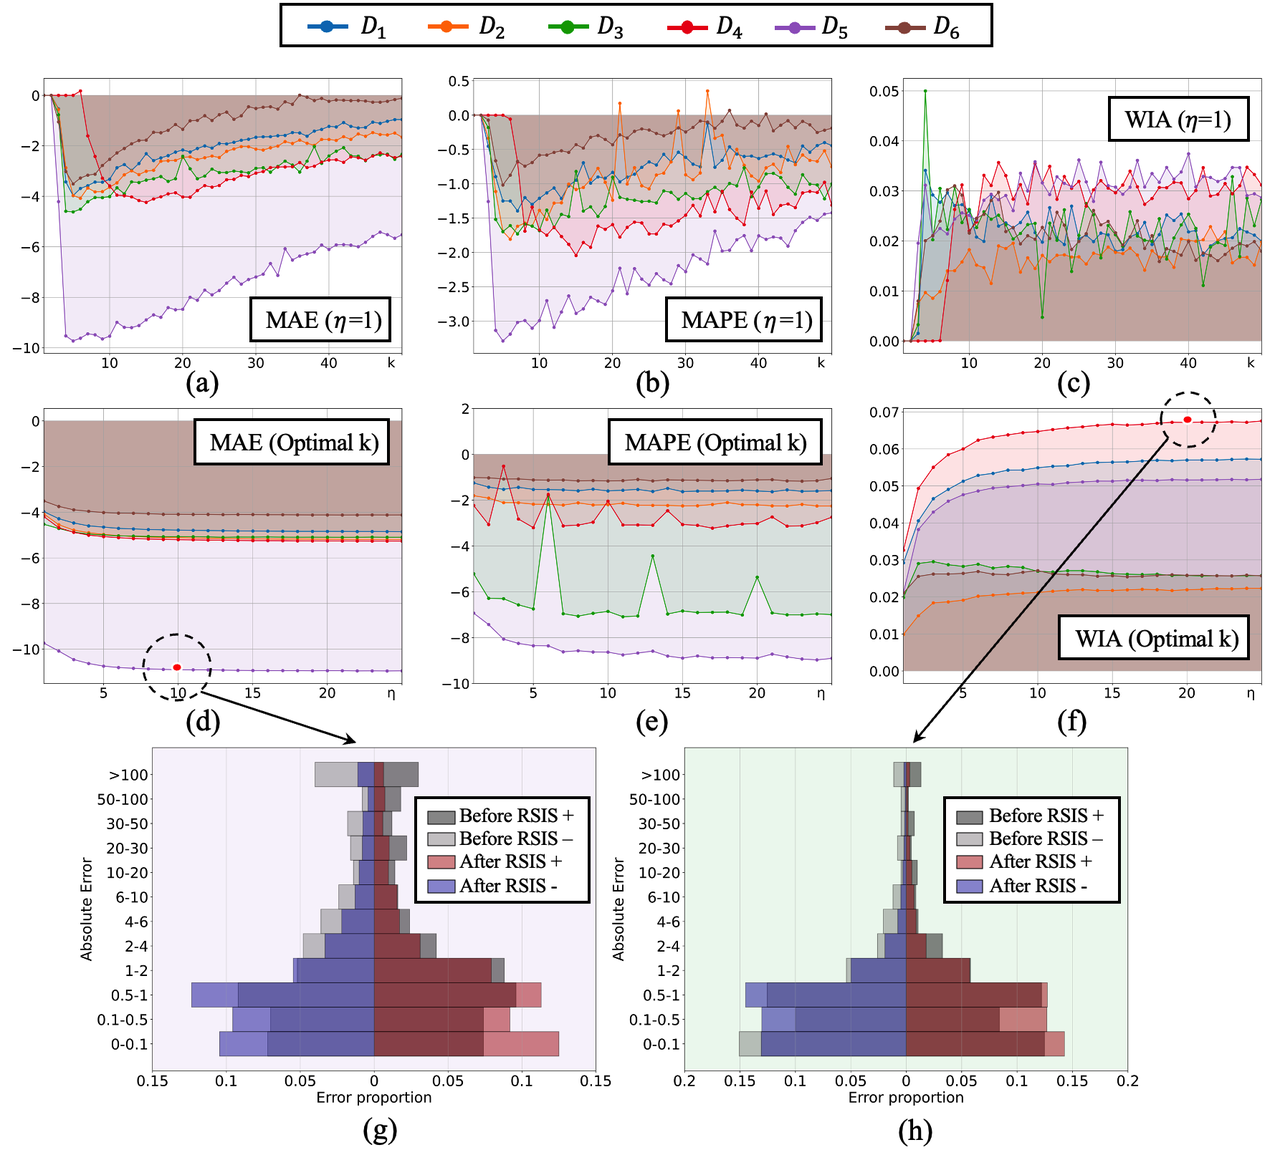
\includegraphics[scale=0.315]{Fig5.png}
  \caption{Optimization effect of the RSIS method with different hyperparameters.}
  \label{Fig5}
\end{figure*}

\subsubsection{Analysis of Optimization Effects}
Table \ref{tab3} presents the results for the MAE (first row), WIA 
(second row), and MAPE (third row) for each simulated experiment's 
original datasets and for the datasets processed using the RSIS 
method under varying hyperparameters. To determine whether the 
datasets were optimized, 
{the Wilcoxon Signed-Rank Test was conducted with a significance level of 0.05 \cite{bib83}.} 
Signs $'+',\;{'-'}\;\text{and}\;{'}{\approx}' $ 
respectively indicate a significant improvement, a significant 
decline, or no significant change in the metrics after processing 
with the RSIS method. The last three rows of the table detail the 
outcomes of the sign rank test, with each tuple representing the 
count of significant results for the respective metric.




Based on the results of the Wilcoxon Signed-Rank Test, it is 
evident that the RSIS method has improved performance across 
nearly all metrics for given datasets, with no instances of 
significant decline observed. For dataset $D_4$ under the 
conditions of $k=5,\eta=1,5,10$, no significant changes were 
noted. This is primarily attributed to the fact that as feature 
dimensionality increases, the samples of most clusters become too 
sparsely distributed in the feature space. During the KNN 
optimization phase, all samples were merged into a single cluster, 
omitting the subsequent phase of RSIS. However, this issue was 
mitigated with an increase in $k$. 




Compared to $\eta$, the optimization effect of the RSIS method 
is more sensitive to the hyperparameter $k$, which will be 
further substantiated in the subsequent section. With an 
appropriately selected value for $k$, elevating the value of 
$\eta$ may amplify the method's optimization efficacy.

Experimental results also show that RSIS's performance continues 
to optimize effectively, as the content of noise with large 
variances increases. Hence, it can deal with more complex noise 
and has good robustness. Moreover, the RSIS method is capable of 
significantly optimizing samples even in datasets with 
heavy-tailed distributions or smaller sample sizes, demonstrating 
its excellent adaptability. 







\subsubsection{Hyperparameter Analysis}
To more clearly demonstrate the optimization effect of RSIS and 
the impact of hyperparameter value, we subtracted the 
pre-optimization metrics from the post-optimization metrics 
and calculated the performance of the simulated datasets under 
various hyperparameters, as shown in Fig. \ref{Fig5}. (a), (b) and (c) 
present the performance of different metrics at various $k$ values 
when $\eta=1$, while (d), (e) and (f) in Fig. \ref{Fig5} display the 
performance across different $\eta$ values at the $k$ value 
where MAE is minimized. 



In the vast majority of cases, all metrics have been optimized. 
Compared to MAE and WIA, MAPE exhibits greater fluctuations. 
The primary reason is the RSIS method synthesizing a substantial 
number of values close to zero. Given that MAPE is particularly 
sensitive to near-zero true values, especially for the simulated 
dataset $D_3$, this leads to larger variations in MAPE.

The performance of each metric under different hyperparameter 
$\eta$ values is more stable compared to $k$, and in most cases, 
as the value of $\eta$ increases, the optimization effect is 
further enhanced, subsequently leading to a gradual stabilization. 
Under different values of $k$, the optimization effect of MAE 
presents a U-shape; MAPE is optimized in most scenarios; and 
WIA initially increases and then fluctuates slightly within a 
stable range.

(g) and (h) in Fig. \ref{Fig5} represent the proportion of errors 
of different magnitudes to the total sample size before and after 
optimization by the RSIS method, with the left part of the graph 
illustrating the proportion of negative errors and the right part 
showing the proportion of positive errors. It is evident that the 
proportion of samples with larger errors has significantly 
decreased following optimization by the RSIS method, while the 
proportion of samples with smaller errors has significantly 
increased. 

{In summary, our experimental results further validate that the RSIS method can effectively increase data diversity and representativeness, and highlight the true functional relationships between variables by synthesizing a large number of samples with smaller errors.}


\subsection{Benchmark Datasets}
To assess the optimization performance in prediction of the RSIS 
method, four benchmark datasets were utilized \cite{bib84,bib85,bib86,bib87}. Samples 
were randomly selected in varying quantities from each dataset 
and divided into training and testing sets. Following 
processing of the training data with the RSIS approach, a 
suite of machine learning models was subsequently trained on 
this dataset,
{which included the original training data as well as the data synthesized by RSIS.}
 The models' predictive performance were subsequently 
assessed on the testing set. For each set of experiments, we 
repeated the process 25 times and took the average value as the 
experimental result, and a Wilcoxon signed-rank test was 
conducted thereafter. In addition, we removed features that 
cannot be directly used, such as “Datetime” for Bike Sharing 
Demand, “Month” for Forest Fires, and so on. We selected a range 
of machine learning models for prediction, including KNN, 
Gradient Boosting Decision Tree (GBDT), Multilayer Perceptron 
(MLP), and Support Vector Regression (SVR), with SVR employing a 
Radial Basis Function (RBF) kernel. 



The computational results for the four models applied to the 
benchmark datasets are presented in Table 4, including the MAE 
and MAPE (in brackets) for each testing set. RSIS consistently 
delivers strong performance across various benchmarks and 
demonstrates exceptional adaptability with different models, 
generally improving their prediction accuracy. It can also be 
seen from Table \ref{tab4} that the effects of normalization 
and the varied sizes of training sets do not impact the 
optimization efficacy of RSIS. Fig. \ref{Fig6} demonstrates 
that after processing with the RSIS method, the prediction outcomes 
of each model are closer to the actual values, and even poorly 
performing prediction models (such as SVR) still achieve a 
significant improvement in predictive performance. 


It is worth mentioning that the dataset contains many variables 
which are not continuous. Moreover, for sparse datasets 
(Facebook Metrics and Forest Fires), it is difficult to guarantee 
that the linear fitting error $\varepsilon'\rightarrow0$ when 
interpolating between subspaces. This indicates that even if there 
are violations of the RSIS assumptions in practical applications, 
this method may still achieve good optimization results. 

 
 

% --------------------------------------------------------------------
% \newpage
\begin{sidewaystable}[htbp]
  \renewcommand{\arraystretch}{0.7}
  \caption{{Experimental} results for benchmark datasets.}\label{tab4}
  \begin{tabularx}{\textwidth}{cccXXXX}
  \toprule
  \multirow{2}{*}{Datasets} & \multirow{2}{*}{Optimizing} & \multirow{2}{*}{$\begin{aligned}&\text{Training\;(Testing)}\\&\qquad\quad\text{set\;size}\end{aligned}$} & \multicolumn{4}{c}{Models} \\ 
  \cmidrule{4-7}
    &  &  & KNN & MLP & SVR & GBDT \\
  \cmidrule{1-7}
  \multirow{6}{*}{$\begin{aligned}&\text{Bike Sharing}\\&\quad\text{Demand}\end{aligned}$} & \multirow{3}{*}{-} & 500 (1000) & 5.99 (0.16) & 2.31 (0.14) & 64.33 (2.34) & 5.25 (0.05) \\
    &  & 1000 (1000) & 4.44 (0.12) & 1.65 (0.12) & 42.98 (1.44) & 4.45 (0.04) \\
    &  & 2000 (1000) & 3.66 (0.11) & 0.47 (0.02) & 26.85 (0.99) & 3.37 (0.04) \\
  \cmidrule{2-7}
    & \multirow{3}{*}{RSIS} & 500 (1000) & 3.66$+$ (0.14$+$) & 0.29$+$ (0.02$+$) & 12.27$+$ (1.44$+$) & 2.92$+$ (0.05$\approx$) \\
    &  & 1000 (1000) & 2.94$+$ (0.12$\approx$) & 0.18$+$ (0.01$+$) & 8.32$+$ (0.83$+$) & 2.94$+$ (0.05$\approx$) \\
    &  & 2000 (1000) & 2.66$+$ (0.09$+$) & 0.15$+$ (0.006$+$) & 4.74$+$ (0.34$+$) & 2.45$+$ (0.04$\approx$) \\
  \cmidrule{1-7}
  \multirow{6}{*}{Air Quality} & \multirow{3}{*}{-} & 500 (1000) & 105.38 (0.12) & 104.23 (0.12) & 327.52 (0.52) & 95.38 (0.11) \\
    &  & 1000 (1000) & 101.86 (0.11) & 98.97 (0.11) & 306.72 (0.49) & 89.29 (0.10) \\
    &  & 2000 (1000) & 95.76 (0.11) & 92.80 (0.10) & 268 (0.44) & 89.24 (0.10) \\
  \cmidrule{2-7}
    & \multirow{3}{*}{RSIS} & 500 (1000) & 101.43$+$ (0.11$+$) & 89.85$+$ (0.10$+$) & 218.93$+$ (0.31$+$) & 89.92$+$ (0.10$+$) \\
    &  & 1000 (1000) & 96.52$+$ (0.11$\approx$) & 88.77$+$ (0.10$+$) & 174.02$+$ (0.30$+$) & 87.52$+$ (0.10$\approx$) \\
    &  & 2000 (1000) & 90.24$+$ (0.10$+$) & 86.18$+$ (0.10$\approx$) & 144.60$+$ (0.20$+$) & 84.18$+$ (0.09$+$) \\
  \cmidrule{1-7}
  \multirow{6}{*}{$\begin{aligned}&\text{Facebook\;Metrics}\\&\;\;\;\text{(Normalized)} \end{aligned}$} & \multirow{3}{*}{-} & 100 (200) & 0.079 (0.189) & 0.072 (0.162) & 0.101 (0.187) & 0.004 (0.013) \\
    &  & 200 (200) & 0.065 (0.152) & 0.070 (0.112) & 0.084 (0.148) & 0.002 (0.006) \\
    &  & 300 (200) & 0.051 (0.124) & 0.055 (0.098) & 0.077 (0.141) & 0.001 (0.004) \\
  \cmidrule{2-7}
    & \multirow{3}{*}{RSIS} & 100 (200) & 0.078$\approx$ (0.181$+$) & 0.061$+$ (0.102$+$) & 0.105$-$ (0.198$-$) & 0.002$+$ (0.007$+$) \\
    &  & 200 (200) & 0.067$-$ (0.151$\approx$) & 0.048$+$ (0.093$+$) & 0.086$-$ (0.153$-$) & 0.001$+$ (0.004$+$) \\
    &  & 300 (200) & 0.056$-$ (0.125$\approx$) & 0.030$+$ (0.053$+$) & 0.076$\approx$ (0.136$+$) & 0.001$\approx$ (0.003$\approx$) \\
  \cmidrule{1-7}
  \multirow{6}{*}{$\begin{aligned}&\text{Forest\;Fires}\\&\text{(Normalized)}\end{aligned}$} & \multirow{3}{*}{-} & 50 (200) & 0.064 (0.540) & 0.177 (0.169) & 0.093 (0.083) & 0.063 (0.053) \\
    &  & 150 (200) & 0.060 (0.055) & 0.161 (0.158) & 0.080 (0.076) & 0.058 (0.054) \\
    &  & 300 (200) & 0.050 (0.039) & 0.093 (0.081) & 0.076 (0.067) & 0.055 (0.044) \\
  \cmidrule{2-7} 
    & \multirow{3}{*}{RSIS} & 50 (200) & 0.062$+$ (0.052$+$) & 0.144$+$ (0.104$+$) & 0.124$-$ (0.114$-$) & 0.077$-$ (0.066$-$) \\
    &  & 150 (200) & 0.059$\approx$ (0.054$\approx$) & 0.058$+$ (0.054$+$) & 0.082$\approx$ (0.078$\approx$) & 0.056$+$ (0.052$+$) \\
    &  & 300 (200) & 0.048$+$ (0.037$+$) & 0.068$+$ (0.057$+$) & 0.073$+$ (0.063$+$) & 0.054$\approx$ (0.043$\approx$) \\
  \cmidrule{1-7}
    & $+$ &  & 8 (7) & 12 (11) & 7 (8) & 9 (5) \\
    & $-$ &  & 2 (0) & 0 (0) & 3 (3) & 1 (1) \\
    & $\approx$ &  & 2 (5) & 0 (1) & 2 (1) & 2 (6) \\
  \bottomrule
  \end{tabularx}
\end{sidewaystable}

\begin{figure}[h!]
  \centering
  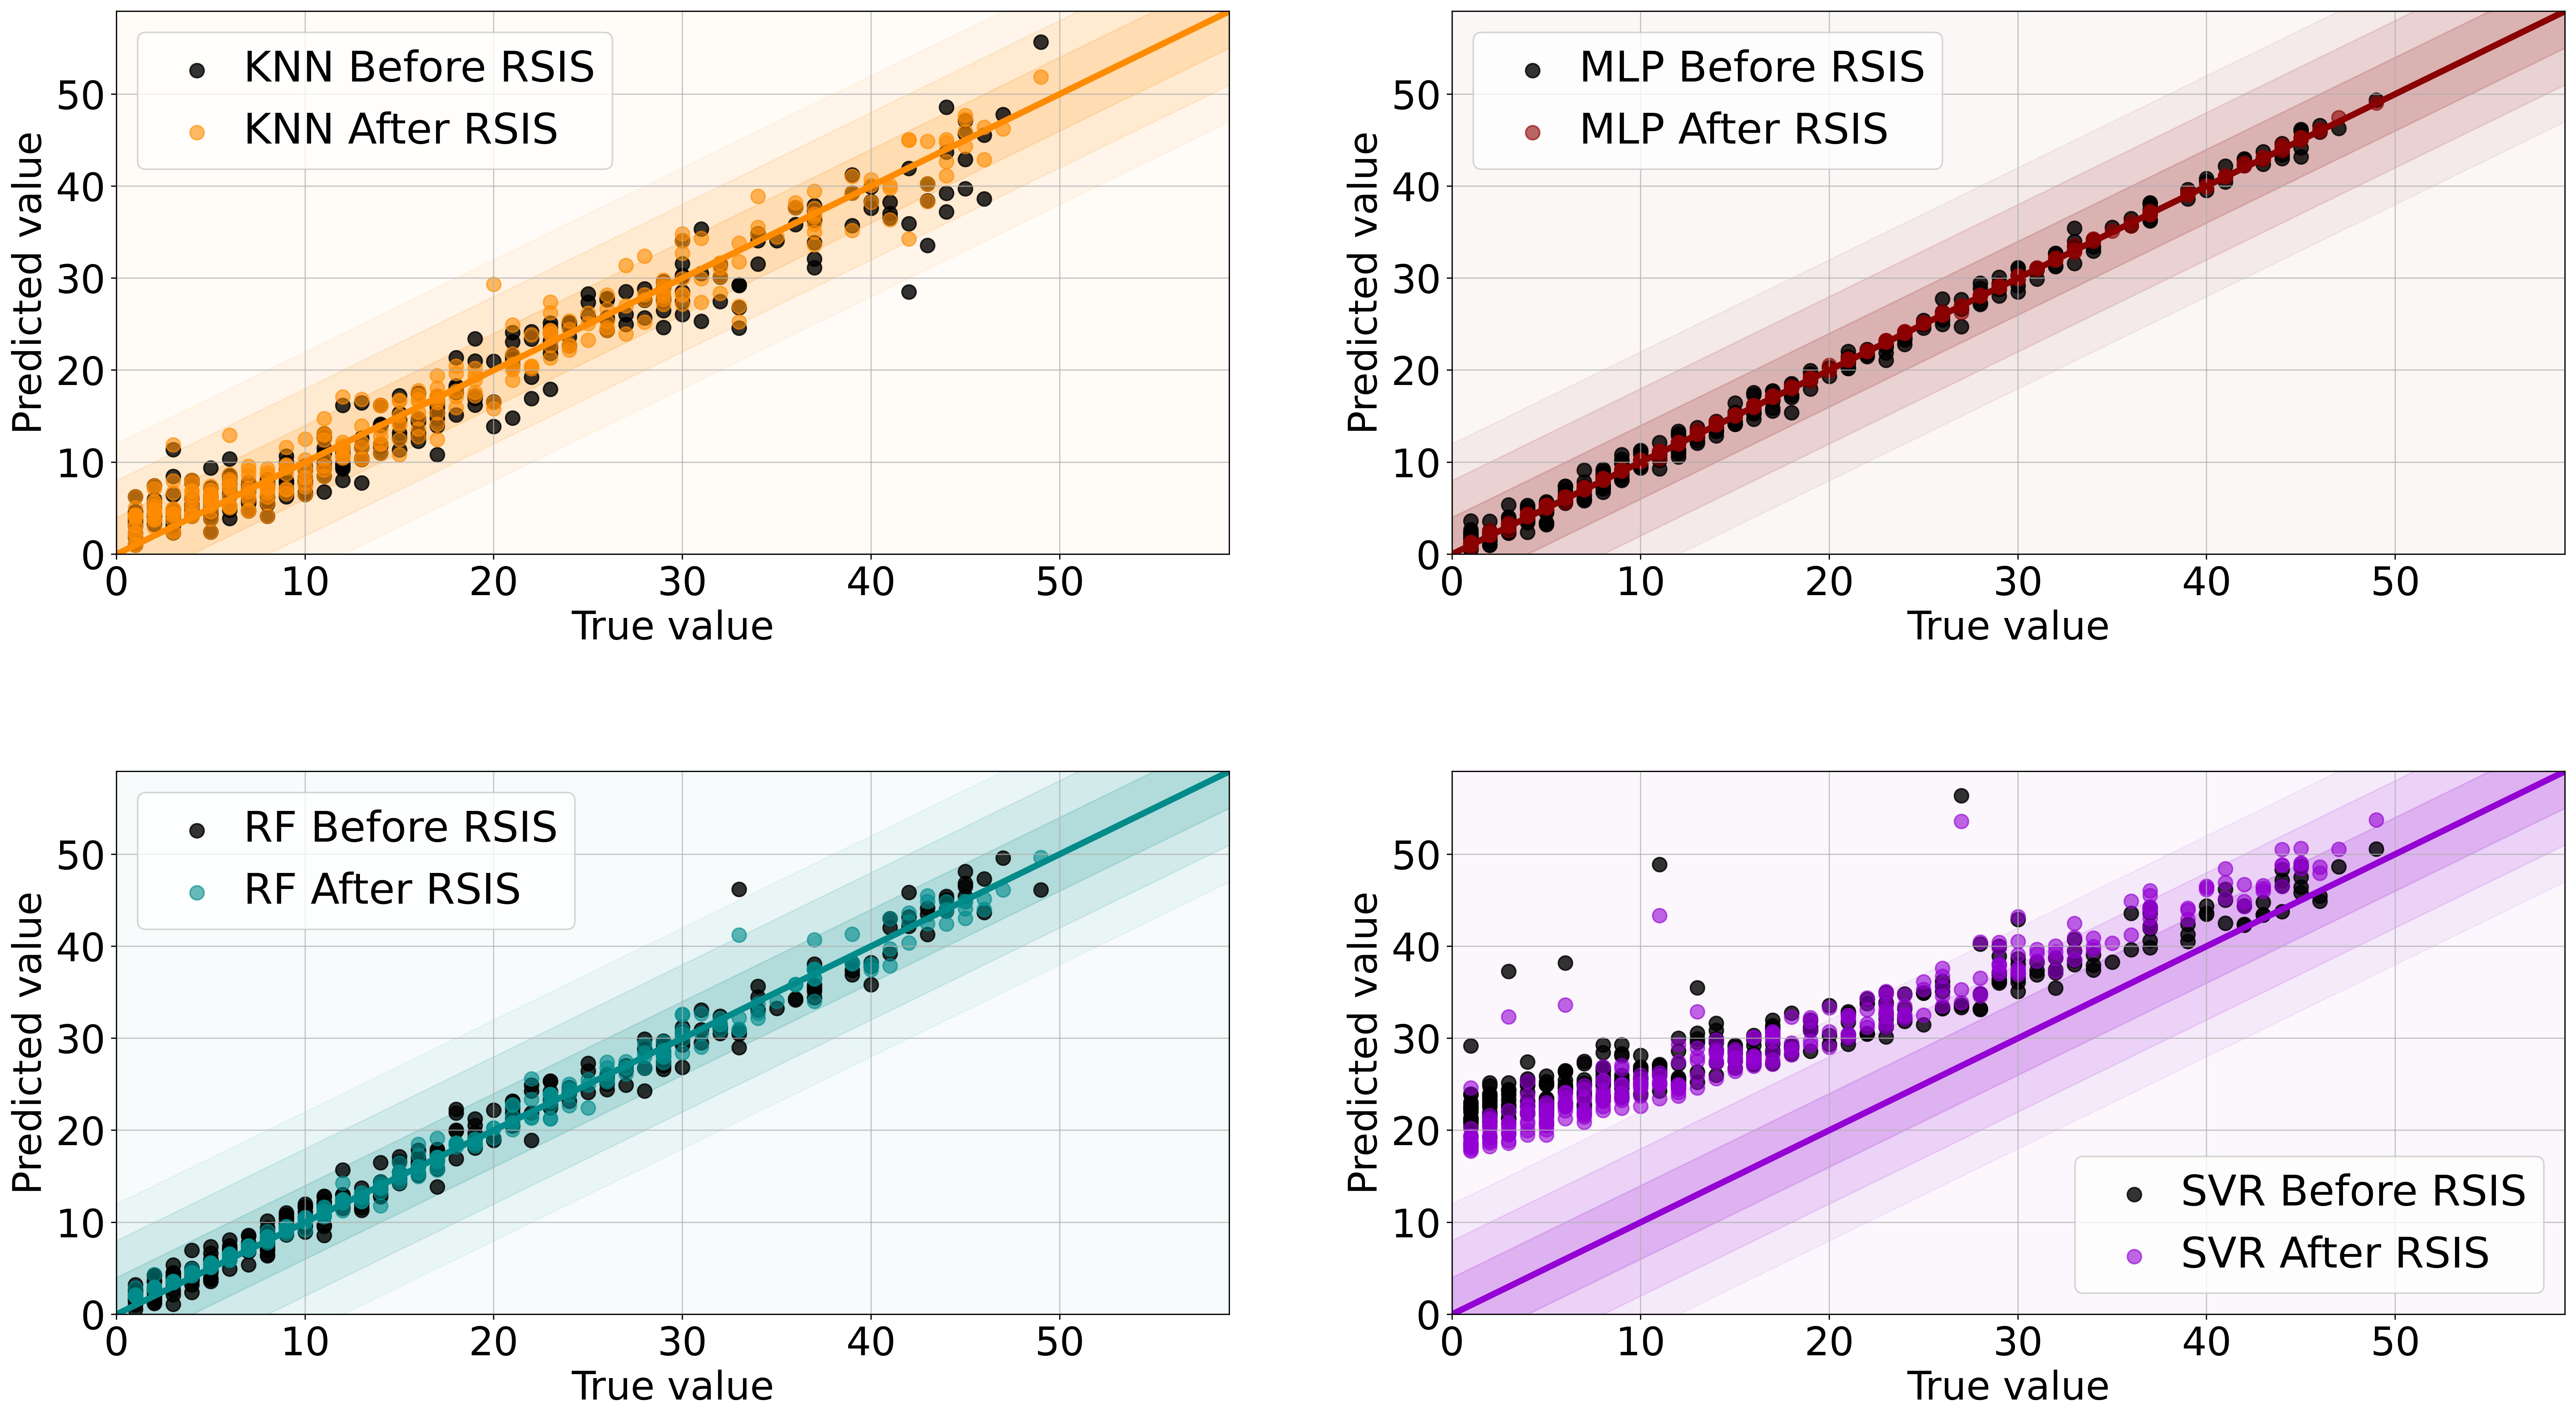
\includegraphics[scale=0.28]{Fig6.png}
  \caption{Comparison of prediction effects on the partly testing 
  set of Bike Sharing Demand.}
  \label{Fig6}
\end{figure}





\newpage
\section{Further Research on CNN Integration}
The preceding research primarily focused on synthesizing data 
using RSIS for feature vector data. This chapter delves into the 
application of the RSIS method in combination with the CNN 
framework in the field of image prediction.


\subsection{Method Overview}
Consider a dataset of RGB images $D=\{\boldsymbol{I}_i,\boldsymbol{L}_i \}_
{i=1}^n$, where $\boldsymbol{L}_i$ is the one-hot vector representing the category of $\boldsymbol{I}_i$. Let the feature extraction function of a CNN be 
$f:\mathbb{R}^{H\times W\times C}\rightarrow \mathbb{R}^d$, 
where $H\times W\times C$ denotes the dimensions and channel 
number of the image, and $d$ represents the dimension of the 
extracted features. Through the feature extraction operation of 
CNN, an image $\boldsymbol{I}_i$ is transformed into a feature 
vector $\boldsymbol{v}_i=f(\boldsymbol{I}_i)$. Using the RSIS 
method, we obtain $\{\boldsymbol{v}_i,\boldsymbol{L}_i\}_{i=1}^{n^\prime}$, 
where $n^\prime$ is the sample size after adding synthesized 
feature vectors. Finally, all samples are placed into a fully 
connected network for iterative training. 

The combination of the RSIS method with the CNN framework 
necessitates changes to traditional model training approaches. 
Consequently, we have designed a two-stage training strategy, as 
illustrated in Fig. \ref{Fig7}.

In the first stage, following traditional training protocols, 
the model performs forward propagation and calculates loss using 
input images. It then uses backpropagation to calculate gradients 
for updating model parameters, continuing this process until 
convergence.

In the second stage, original images are processed by the feature 
extractor, trained in the initial stage, to generate a dataset of 
feature vectors for each image. Subsequently, the RSIS method is 
employed on this dataset to synthesize new data, which is then 
exclusively retrained in the fully connected layer until 
convergence is reached. Notably, this stage updates only the 
fully connected layer's parameters, leaving the feature extraction 
layers unchanged during the training process.

\begin{figure}[h!]
  \centering
  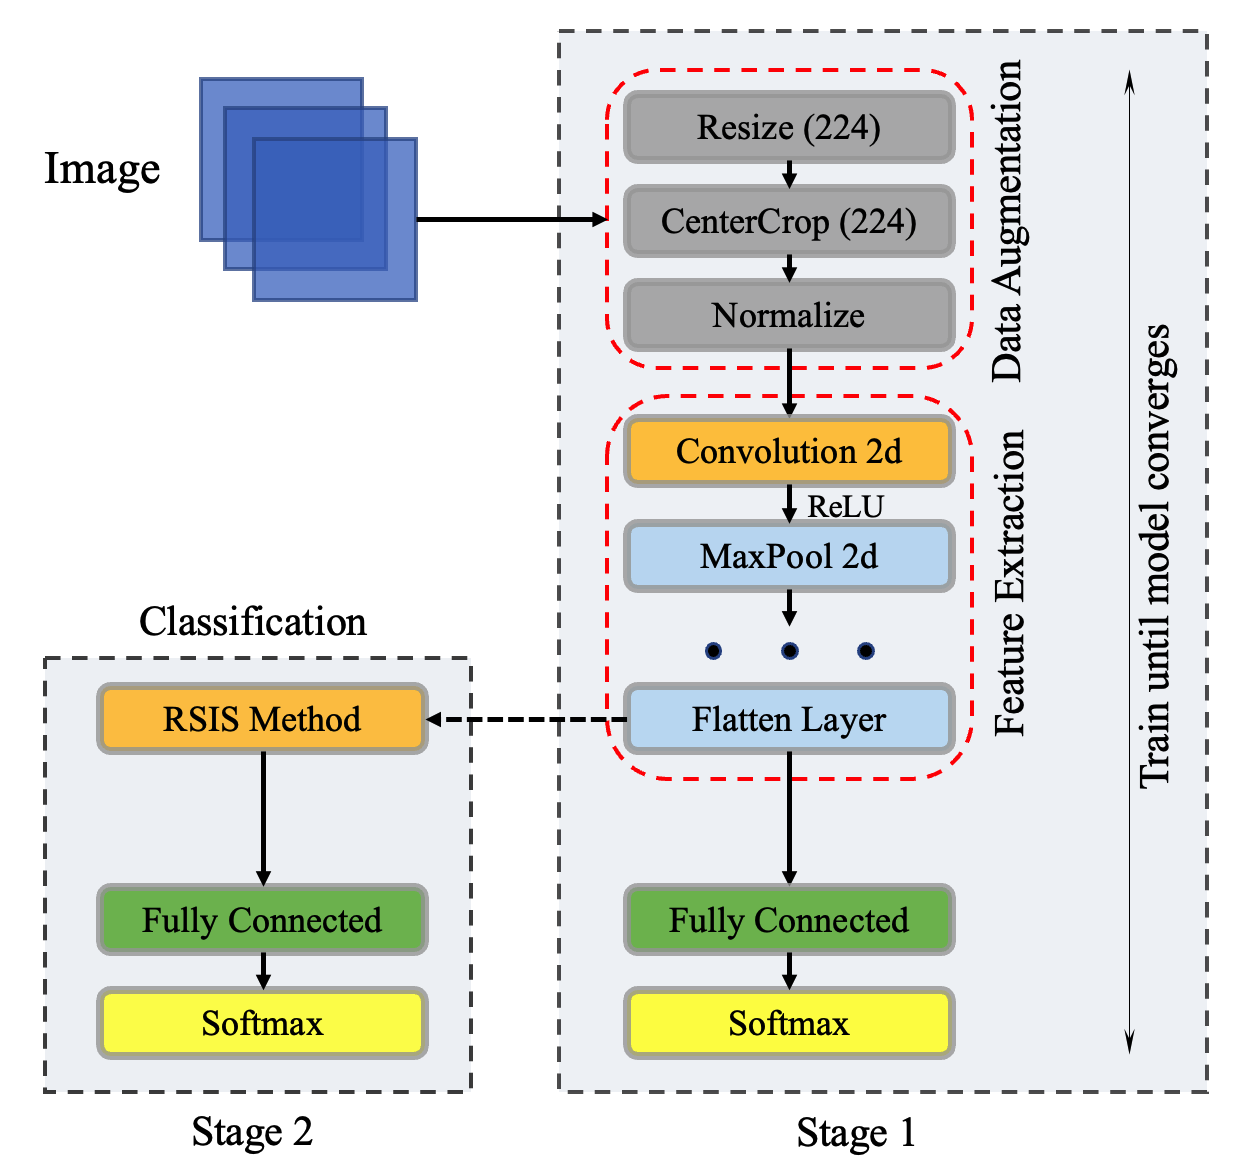
\includegraphics[width=4.6in]{Fig7.png}
  \caption{RSIS method combined with CNN framework.}
  \label{Fig7}
\end{figure}


\subsection{Analysis of Optimization Effects}
To assess the optimization performance in prediction, four 
image datasets (MNIST \cite{bib88}, FashionMNIST \cite{bib89}, CIFAR-10 \cite{bib90}, and 
SVHN \cite{bib91}) and CNN frameworks were utilized, including ResNet50, 
VGG16, DenseNet121, and MobileNet-v2. All models were initialized 
with pre-trained parameters. We randomly selected 200 and 1,000 
samples as the training and testing sets, respectively. In the 
second stage, new synthesized samples were added to the training 
set, expanding the original dataset to 500, 1,000, and 3,000 
samples to explore the optimization effects at different scales. 
The process was repeated 25 times, with the average value taken 
as the experimental result, followed by a Wilcoxon signed-rank 
test. The optimization effect of the RSIS method was measured by 
the variation in the test error rate $E_{\text{var}}$:
\begin{equation}
\label{eq19}
  E=\dfrac{1}{n}\sum\limits_{i=1}^n{I}(\hat{L}_i\neq L_i),
\end{equation}
\begin{equation}
\label{eq20}
  E_{\text{var}}=E_{\text{stage1}}-E_{\text{stage2}},
\end{equation}
where $E_{\text{stage1}}$ represents the error rate on the testing 
set at the end of the first stage, and $E_{\text{stage2}}$ is 
the error rate post the second stage. It can be seen from Table \ref{tab5} 
that the RSIS significantly enhances the model's generalization 
capability in most cases. However, the benefits derived from the 
RSIS method vary according to the model's adaptability and 
compatibility with specific datasets. For instance, DenseNet121 
demonstrates significant generalization improvement and a 
pronounced reduction in prediction errors on the SVHN dataset.

\begin{table}[t!]
  \centering
  \begin{threeparttable}
    \caption{Experimenal results for image datasets.}\label{tab5}
  \begin{tabular}{cccccc}
  \toprule
  \multirow{2}{*}{Models} & \multirow{2}{*}{After RSIS} & \multicolumn{4}{c}{Datesets}  \\ 
  \cmidrule{3-6}
    &  & MNIST & FashionMNIST & CIFAR-10 & SVHN \\
  \cmidrule{1-6}
  \multirow{3}{*}{ResNet50} & 500 & 1.70\%$+$ & 0.30\%$+$ & 0.50\%$+$ & 3.10\%$+$ \\
    & 1000 & 1.90\%$+$ & 1.30\%$+$ & 1.60\%$+$ & 3.60\%$+$ \\
    & 3000 & 2.70\%$+$ & 1.50\%$+$ & 2.10\%$+$ & 3.60\%$+$ \\
  \cmidrule{2-6}
  \multirow{3}{*}{VGG16} & 500 & 0.20\%$+$ & 0.10\%$-$ & 0.30\%$-$ & 0.80\%$-$ \\
    & 1000 & 0.50\%$+$ & 0.90\%$+$ & 0.40\%$+$ & 0.00\%$\approx$ \\
    & 3000 & 0.70\%$+$ & 1.10\%$+$ & 0.40\%$+$ & 0.00\%$\approx$ \\
  \cmidrule{2-6}
  \multirow{3}{*}{DenseNet121} & 500 & 0.70\%$+$ & 0.20\%$+$ & 0.00\%$\approx$ & 4.70\%$+$ \\
    & 1000 & 1.00\%$+$ & 0.30\%$+$ & 0.50\%$+$ & 5.10\%$+$ \\
    & 3000 & 1.70\%$+$ & 0.60\%$+$ & 1.00\%$+$ & 5.40\%$+$ \\
  \cmidrule{2-6}
  \multirow{3}{*}{MobileNet-v2} & 500 & 1.30\%$+$ & 0.70\%$-$ & 0.20\%$+$ & 3.30\%$+$ \\
    & 1000 & 1.50\%$+$ & 0.40\%$+$ & 1.80\%$+$ & 5.20\%$+$ \\
    & 3000 & 1.70\%$+$ & 1.20\%$+$ & 2.50\%$+$ & 5.70\%$+$ \\
  \cmidrule{1-6}
  $+$ &  & 12 & 10 & 10 & 9 \\
  $-$ &  & 0  & 2  & 1  & 1 \\
  $\approx$ &  & 0 & 0 & 1 &2 \\
  \bottomrule
  \end{tabular}
  \end{threeparttable}
\end{table}


We selected the MNIST dataset, and examined the iterative changes 
in $E_{\text{stage2}}$, as illustrated in Fig \ref{Fig8}. The section 
right of the red dashed line illustrates the subsequent iterative 
changes in $E_{\text{stage2}}$ for three distinct synthesized 
sample sizes, following optimization with RSIS. It is evident 
that in most scenarios, the error significantly decreases in the 
second stage.

Fig. \ref{Fig9} presents the predictive performance of four 
models across metrics $\rho_1$ (Misclassification Improvement 
Ratio) and $\rho_2$ (Negative Conversion Rate) on the 
FashionMNIST dataset.
\begin{equation}
\label{eq21}
\rho_1=\dfrac{\text{num}(C_{\text{stage2}}\cap  
M_{\text{stage1}})}{\text{num}(M_{\text{stage1}})},
\end{equation}
\begin{equation}
\label{eq22}
\rho_2=\dfrac{\text{num}(M_{\text{stage2}}\cap C_{\text{stage1}})}
{\text{num}(C_{\text{stage1}})},
\end{equation}
where $M_{\text{stage1}}$ and $M_{\text{stage2}}$ denote the 
sample misclassified sets before and after optimization, while 
$C_{\text{stage1}}$ and $C_{\text{stage2}}$ denote the sample 
correctly sets classified before and after optimization, 
respectively.  In the majority of scenarios, $\rho_1$ tends to 
increase with the growth of synthesized samples in the training 
set, a trend that is particularly pronounced in VGG16 and 
DenseNet121. Conversely, $\rho_2$ generally decreases as the 
training set expands, with this effect being especially notable 
in VGG16. 

\begin{figure}[h!]
  \centering
  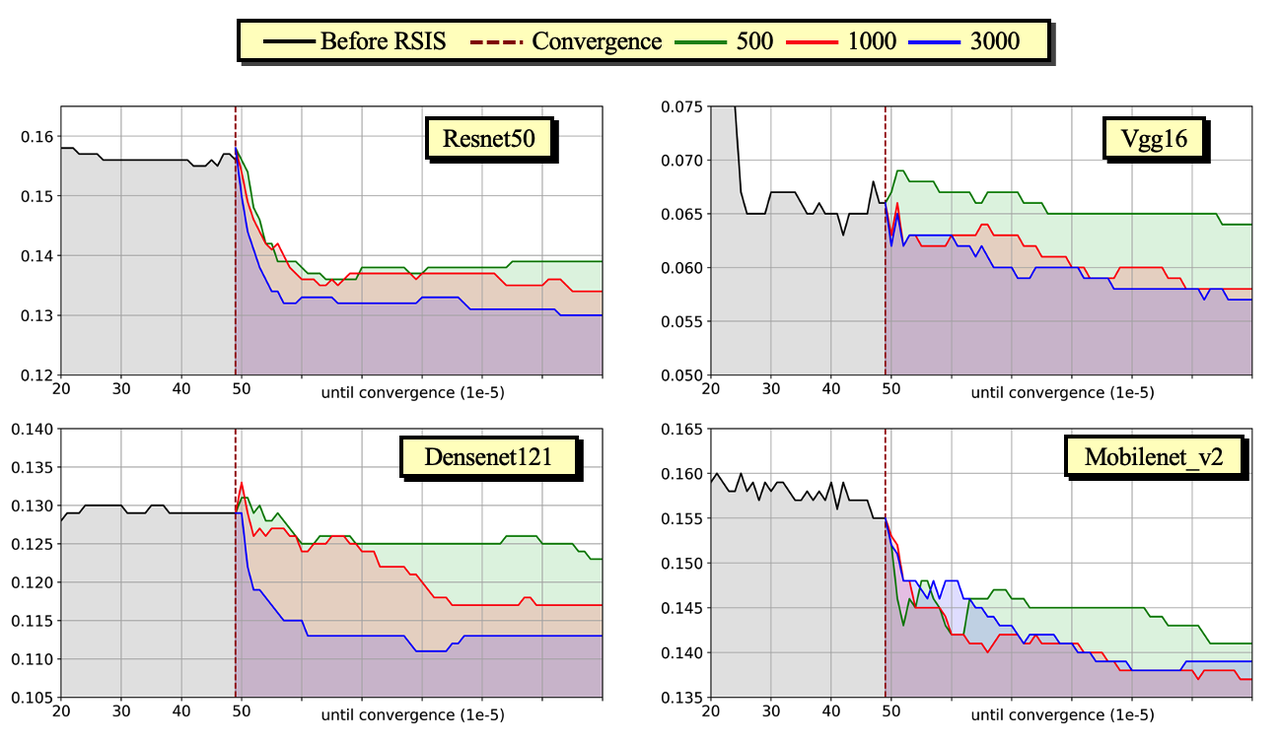
\includegraphics[scale=0.32]{Fig8.png}
  \caption{Iterative comparison of prediction errors.}
  \label{Fig8}
\end{figure}

\begin{figure}[h!]
  \centering
  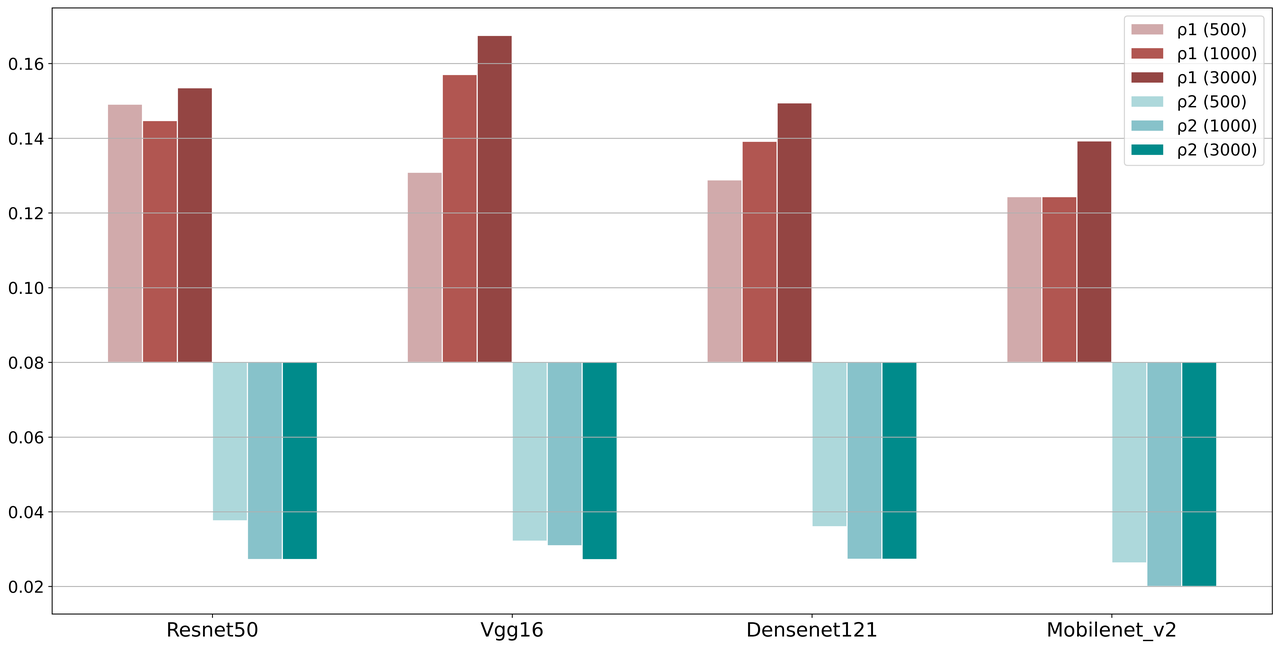
\includegraphics[scale=0.3]{Fig9.png}
  \caption{The predictive performance of four models across metrics $\rho_1$ and $\rho_2$.}
  \label{Fig9}
\end{figure}

% --------------------------------------------------------------------

\section{Conclusion}
This paper introduces a data synthesis method based on linear and 
equidistant interpolation within feature subspaces, which 
synthesizes samples with reduced noise without sacrificing 
the original sample information and adaptively interpolates 
between feature subspaces to enhance data diversity and 
representativeness. Furthermore, our experimental results reveal 
that the RSIS method significantly optimizes samples by 
synthesizing samples with reduced noise and simultaneously 
decreasing the proportion of high-noise samples. On benchmark 
datasets, it notably enhances the models' generalization 
capabilities. By innovatively integrating the RSIS method with 
the convolutional neural network framework, we have further 
improved the model's predictive performance.

{RSIS can also be combined with methods from various fields, such as evolutionary algorithms, serving as a mutation strategy for differential evolution algorithms.} However, RSIS is not suitable for studies on sample distribution because it alters 
the distribution of variables. Theoretically, if {the}
hyperparameter $\eta$ is set to infinity, variables will 
tend to a uniform distribution. Exploring how to significantly 
optimize samples without disrupting their distribution is worth 
pursuing. {Moreover, the requirement of RSIS to flatten image data, i.e., matrix and tensor data, limits its ability to preserve positional information. Future research should address challenges associated with various data types, including heterogeneous and functional data, to enhance diversity while maintaining intrinsic distribution characteristics.}



\section*{CRediT authorship contribution statement}
Yukun Du: Methodology, Writing – original draft. Yitao Cai: Writing – original draft
Software,  Xiao Jin: Writing, Data curation.   Zhilong Lou: Validation, Supervision.  Yao Li: Writing – review Yongxiong Wang: Writing – review. Jiang Jiang: Writing – review. Haiyue Yu:Writing – review.

\section*{Declaration of competing interest}
The authors declare that they have no known competing financial interests or personal relationships that could have appeared to
influence the work reported in this paper.
\section*{Data availability}
No data was used for the research described in the article.
\section*{Funding}
This research was supported by a grant from Natural Science Foundation of Shanghal under Grand 22ZR1443700.



%% The Appendices part is started with the command \appendix;
%% appendix sections are then done as normal sections
%% \appendix

%% \section{}
%% \label{}
\appendix


\section{Proof of Lemma 1}
Consider the function $f(\boldsymbol{\beta})=\|
\boldsymbol{y}-\boldsymbol{X}\boldsymbol{\beta}\|_2^2$, 
where $\|\boldsymbol{y}-\boldsymbol{X}\boldsymbol{\beta}
\|_2$ denotes the $L_2$ norm of $\boldsymbol{y}-
\boldsymbol{X}\boldsymbol{\beta}$. Then, for 
$\forall\omega\in[0,1]$, and $\forall\boldsymbol{\beta}_1,
\boldsymbol{\beta}_2\in\mathbb{R}^{d\times1}$, we have:
\begin{equation*}
\begin{aligned}
  &f(\omega\boldsymbol{\beta}_1+(1-\omega)\boldsymbol{\beta_2})- \omega f(\boldsymbol{\beta_1})-(1-\omega)f(\boldsymbol{\beta_2}) \\
  &=||y-X(\omega\boldsymbol{\beta}_1+(1-\omega)\boldsymbol{\beta}_2)||_2^2-\omega||y-X\boldsymbol{\beta}_1||_2^2-(1-\omega)||y-X\boldsymbol{\beta}_2||_2^2 \\
  &=||\omega y+(1-\omega)y-X(\omega\boldsymbol{\beta}_1+(1-\omega)\boldsymbol{\beta}_2)||_2^2-\omega||y-X\boldsymbol{\beta}_1||_2^2-(1-\omega)||y-X\boldsymbol{\beta}_2||_2^2 \\
  &=||\omega(y-X\boldsymbol{\beta}_1)+(1-\omega)(y-X\boldsymbol{\beta}_2)||_2^2-\omega||y-X\boldsymbol{\beta}_1||_2^2-(1-\omega)||y-X\boldsymbol{\beta}_2||_2^2 \\
  &=\omega^2||y-X\boldsymbol{\beta}_1||_2^2+(1-\omega)^2||y-X\boldsymbol{\beta}_2||_2^2 +2\omega(1-\omega)(y-X\boldsymbol{\beta}_1)^\prime(y-X\boldsymbol{\beta}_2)-\omega||y-X\boldsymbol{\beta}_1||_2^2-(1-\omega)||y-X\boldsymbol{\beta}_2||_2^2 \\
  &=\omega^2||y-X\boldsymbol{\beta}_1||_2^2+(1-2\omega+\omega^2)||y-X\boldsymbol{\beta}_2||_2^2 +(2\omega-2\omega^2)(y-X\boldsymbol{\beta}_1)^\prime(y-X\boldsymbol{\beta}_2)-\omega||y-X\boldsymbol{\beta}_1||_2^2-(1-\omega)||y-X\boldsymbol{\beta}_2||_2^2 \\
  &=\omega^2\left(||y-X\boldsymbol{\beta}_1||_2^2 - 2(y-X\boldsymbol{\beta}_1)^\prime(y-X\boldsymbol{\beta}_2)+||y-X\boldsymbol{\beta}_2||_2^2 \right)+(1-2\omega)||y-X\boldsymbol{\beta}_2||_2^2+2\omega(y-X\boldsymbol{\beta}_1)^\prime(y-X\boldsymbol{\beta}_2)-\\&\omega||y-X\boldsymbol{\beta}_1||_2^2-(1-\omega)||y-X\boldsymbol{\beta}_2||_2^2 \\
  &=\omega^2||(y-X\boldsymbol{\beta}_1)-(y-X\boldsymbol{\beta}_2)||_2^2+2\omega(y-X\boldsymbol{\beta}_1)^\prime(y-X\boldsymbol{\beta}_2)-\omega||y-X\boldsymbol{\beta}_1||_2^2-\omega||y-X\boldsymbol{\beta}_2||_2^2 \\
  &=\omega^2||(y-X\boldsymbol{\beta}_1)-(y-X\boldsymbol{\beta}_2)||_2^2-\omega||(y-X\boldsymbol{\beta}_1)-(y-X\boldsymbol{\beta}_2)||_2^2 \\
  &=\omega(\omega-1)||(y-X\boldsymbol{\beta}_1)-(y-X\boldsymbol{\beta}_2)||_2^2 \le0.
\end{aligned}
\end{equation*}

From inequality $f(\omega\boldsymbol{\beta}_1+(1-\omega)
\boldsymbol{\beta}_2)- \omega f(\boldsymbol{\beta}_1)-
(1-\omega)f(\boldsymbol{\beta}_2)\le0$, simplification 
yields the convexity condition:
\begin{equation*}
\begin{aligned}
f(\omega\boldsymbol{\beta}_1+(1-\omega)\boldsymbol{\beta}_
2)\le \omega f(\boldsymbol{\beta}_1)+(1-\omega)
f(\boldsymbol{\beta}_2).
\end{aligned}
\end{equation*}

\section{Proof of Lemma 2}
Considering the linear structure of $f(\boldsymbol
{\beta})$ with respect to the $L_1$ norm, we commence 
the proof by examining the function at a convex 
combination of $\boldsymbol{\beta}_1$ and $\boldsymbol
{\beta}_2$, and we have:
\begin{equation*}
  \begin{aligned}
    f(\omega\boldsymbol{\beta}_1+(1-\omega)\boldsymbol{\beta}_2)
    &=||(\omega\boldsymbol{\beta}_1^1+(1-\omega)\boldsymbol{\beta}_2^1)-(\omega\boldsymbol{\beta}_1^2+(1-\omega)\boldsymbol{\beta}_2^2)||_1 \\
    &= ||\omega(\boldsymbol{\beta}_1^1-\boldsymbol{\beta}_1^2)+(1-\omega)(\boldsymbol{\beta}_2^1-\boldsymbol{\beta}_2^2)||_1 \\
    &\le \omega||\boldsymbol{\beta}_1^1-\boldsymbol{\beta}_1^2||_1+(1-\omega)||\boldsymbol{\beta}_2^1-\boldsymbol{\beta}_2^2||_1 \\
    &= \omega f(\boldsymbol{\beta}_1)+(1-\omega)f(\boldsymbol{\beta}_2).
  \end{aligned}
\end{equation*}

\section{Proof of Theorem 1}
Let $\lambda_{p,q}=\dfrac{\lambda}{\text{dist}(\overline
{\boldsymbol{x}}^{p},\overline{\boldsymbol{x}}^{q})+1}$, 
$L(\boldsymbol{\beta})=\gamma_1(\boldsymbol{\beta})+
\gamma_2(\boldsymbol{\beta})$, where
\begin{equation*}
\begin{aligned}
\gamma_1(\boldsymbol{\beta})=\sum\limits_{s=2}^
{k^\prime-1}\lambda_{s,s-1}L_1(\boldsymbol{\beta}^{s,s+1},
\boldsymbol{\beta}^{s-1,s}) +\lambda_{k^\prime,1}L_1
(\boldsymbol{\beta}^{1,2},\boldsymbol{\beta}^{k^\prime,1}) +\lambda_{k^\prime-1,k^\prime}L_1(\boldsymbol{\beta}^{k^\prime,1},
  \boldsymbol{\beta}^{k^\prime-1,k^\prime}),
\end{aligned}
\end{equation*}
\begin{equation*}
\gamma_2(\boldsymbol{\beta})=\sum\limits_{s=1}^
{k^\prime-1}L_2(\boldsymbol{\beta}^{s,s+1})+
L_2(\boldsymbol{\beta}^{k^\prime,1}),
\end{equation*}
we have: 
\begin{equation*}
\begin{aligned}
L(\omega\boldsymbol{\beta}_1+(1-\omega)\boldsymbol{\beta}_2)=\gamma_1(\omega\boldsymbol{\beta}_1+(1-\omega)\boldsymbol
{\beta}_2)+\gamma_2(\omega\boldsymbol{\beta}_1+(1-\omega)
\boldsymbol{\beta}_2).
\end{aligned}
\end{equation*}

Based on Lemma 1 and Lemma 2, we obtain:
\begin{equation*}
\begin{aligned}
L_1(\omega\boldsymbol{\beta}^{q,r}_1+(1-\omega)
\boldsymbol{\beta}^{q,r}_2,\omega\boldsymbol{\beta}^
{p,q}_1+(1-\omega)\boldsymbol{\beta}^{p,q}_2)\le\omega L_1(\boldsymbol{\beta}^{q,r}_1,\boldsymbol
{\beta}^{p,q}_1)+(1-\omega)L_1(\boldsymbol{\beta}_2^{q,r},
\boldsymbol{\beta}^{p,q}_2),
\end{aligned}
\end{equation*}
\begin{equation*}
L_2(\omega\boldsymbol{\beta}^{p,q}_1+(1-\omega)
\boldsymbol{\beta}^{p,q}_2)\le\omega L_2
(\boldsymbol{\beta}^{p,q}_1)+(1-\omega)L_2
(\boldsymbol{\beta}^{p,q}_2),
\end{equation*}
which further implies:
\begin{equation*}
\begin{aligned}
&\gamma_1(\omega\boldsymbol{\beta}_1+(1-\omega)\boldsymbol
{\beta}_2) \\
&\le \sum\limits_{s=2}^{k^\prime-1}\lambda_{s,s-1}
(\omega L_1(\boldsymbol{\beta}^{s,s+1}_1,\boldsymbol
{\beta}^{s-1,s}_1)+(1-\omega)L_1(\boldsymbol{\beta}_2^
{s,s+1},\boldsymbol{\beta}^{s-1,s}_2))+\lambda_{k^\prime,1}(\omega L_1(\boldsymbol{\beta}^{1,2}
_1,\boldsymbol{\beta}^{k^\prime,1}_1)+(1-\omega)L_1(\boldsymbol{\beta}_2^{1,2},\boldsymbol{\beta}^
{k^\prime,1}_2)) \\
&=\omega\gamma_1(\boldsymbol{\beta}_1)+(1-\omega)\gamma_1
(\boldsymbol{\beta}_2),
\end{aligned}
\end{equation*}
\begin{equation*}
\begin{aligned}
\gamma_2(\omega\boldsymbol{\beta}_1+(1-\omega)\boldsymbol{\beta}_2)
&\le\sum\limits_{s=1}^{k^\prime-1}(\omega L_2(\boldsymbol{\beta}^{s,s+1}_1)+(1-\omega)L_2(\boldsymbol{\beta}^{s,s+1}_2))+\omega L_2(\boldsymbol{\beta}^{k^\prime,1}_1)+(1-\omega)L_2(\boldsymbol{\beta}^{k^\prime,1}_2) \\
&=\omega\gamma_2(\boldsymbol{\beta}_1)+(1-\omega)\gamma_2(\boldsymbol{\beta}_2).
\end{aligned}
\end{equation*}

Hence, we have:
\begin{equation*}
\begin{aligned} 
L(\omega\boldsymbol{\beta}_1+(1-\omega)\boldsymbol{\beta}_2) 
&=\gamma_1(\omega\boldsymbol{\beta}_1+(1-\omega)\boldsymbol{\beta}_2)+\gamma_2(\omega\boldsymbol{\beta}_1+(1-\omega)\boldsymbol{\beta}_2) \\
&\le \omega\gamma_1(\boldsymbol{\beta}_1)+(1-\omega)\gamma_1(\boldsymbol{\beta}_2)+\omega\gamma_2(\boldsymbol{\beta}_1)+(1-\omega)\gamma_2(\boldsymbol{\beta}_2) \\
&=\omega L(\boldsymbol{\beta}_1)+(1-\omega)L(\boldsymbol {\beta}_2). \end{aligned}
\end{equation*}

\section{Proof of Theorem 2}
Since $\varepsilon^\prime\rightarrow0$, it follows from 
Equation \ref{eq7} that:
\begin{equation*}
y^{s,s+1}=g_{s,s+1}(x^{s,s+1})+\varepsilon.
\end{equation*}

Transform Equation \ref{eq12} to:
\begin{equation*}
\bar{S}(x^s,x^{s+1})=\frac{\int_{x^s}^{x^{s+1}}|g(x)-l(x)|
 dx}{|x^{s+1}-x^s|}.
\end{equation*}

According to the Law of Iterated Expectations(LIE):
\begin{equation*}
\begin{aligned}
\mathbb{E}(\bar{S}(x^s,x^{s+1}))
=\mathbb{E}(\bar{S}(x^s,x^{s+1})|\varepsilon^s\cdot\varepsilon^{s+1}<0)P(\varepsilon^s\cdot\varepsilon^{s+1}<0) +\mathbb{E}(\bar{S}(x^s,x^{s+1})|\varepsilon^s\cdot\varepsilon^{s+1}\ge0)P(\varepsilon^s\cdot\varepsilon^{s+1}\ge0).
\end{aligned}
\end{equation*}

We can simplify $\bar{S}(x^s,x^{s+1})$ using basic 
geometric area calculations. If $\varepsilon^s\cdot
\varepsilon^{s+1}<0$, then $\exists\; x^\prime\in
(x^s,x^{s+1})$, such that $g(x^\prime)=l(x\prime)$. 
It follows that:
\begin{equation*}
\begin{aligned}
\mathbb{E}(\bar{S}(x^s,x^{s+1})|\varepsilon^s\cdot
\varepsilon^{s+1}<0)
=\frac{\mathbb{E}(|\varepsilon^s|)
\cdot|x^s-x'|+\mathbb{E}(|\varepsilon^{s+1}|)\cdot
|x^{s+1}-x'|}{2|x^{s+1}-x^s|}.
\end{aligned}
\end{equation*}

If $\varepsilon^s\cdot\varepsilon^{s+1}\ge0$, then
\begin{equation*}
\begin{aligned}
\mathbb{E}(\bar{S}(x^s,x^{s+1})|\varepsilon^s\cdot
\varepsilon^{s+1}\ge0)
&=\frac{\mathbb{E}(|\varepsilon^s|+
|\varepsilon^{s+1}|)\cdot|x^{s+1}-x^{s}|}
{2|x^{s+1}-x^s|}\\
&=\frac{\mathbb{E}(|\varepsilon^s|+|\varepsilon^{s+1}|)}
{2}.
\end{aligned}
\end{equation*}

Substituting into the original formula, it can be derived:
\begin{equation*}
\begin{aligned}
\mathbb{E}({\bar{S}(x^{s}, x^{(s+1)})})
=\frac{{\mathbb{E}(|\varepsilon^s|)\cdot|x^s-x'|+
\mathbb{E}(|\varepsilon^{s+1}|)\cdot|x^{s+1}-x'|}}
{2|x^{s+1}-x^s|}P(\varepsilon^s\cdot\varepsilon^{s+1}<0)+\frac{\mathbb{E}(|\varepsilon^s|+|\varepsilon^
{s+1}|)}{2}P(\varepsilon^s\cdot\varepsilon^{s+1}\ge0).
\end{aligned}
\end{equation*}

Note that $P(\varepsilon^s\cdot\varepsilon^{s+1}<0)+
P(\varepsilon^s\cdot\varepsilon^{s+1}\ge0)=1$, and
\begin{equation*}
\begin{aligned}
\frac{{\mathbb{E}(|\varepsilon^s|)\cdot|x^s-x'|+
\mathbb{E}(|\varepsilon^{s+1}|)\cdot|x^{s+1}-x'|}}
{2|x^{s+1}-x^s|} 
&=\frac{{\mathbb{E}(|\varepsilon^s|)\cdot|\frac{x^s-x'}
{x^{s+1}-x^s}|+\mathbb{E}(|\varepsilon^{s+1}|)\cdot|
\frac{x^{s+1}-x'}{x^{s+1}-x^s}|}}{2}\\
&<\frac{{\mathbb{E}(|\varepsilon^s|)+\mathbb{E}(|
\varepsilon^{s+1}|)}}{2},
\end{aligned}
\end{equation*}
imply that:
\begin{equation*}
\mathbb{E}(\bar{S}(x^s,x^{s+1}))<\mathbb{E}(\frac{|
\varepsilon^s|+|\varepsilon^{s+1}|}{2}).
\end{equation*}

\section{Proof of Theorem 3}
If $\varepsilon^s\cdot\varepsilon^{s+1}<0$, then $\exists
\;x'\in(x^s,x^{s+1})$, such that $g(x')=l(x')$. It follows 
that:
\begin{equation*}
\begin{aligned}
\bar{S}(x^s,x^{s+1})
&=\frac{|\varepsilon^{s}|\cdot|x^{s}-x'|+|\varepsilon^
{s+1}|\cdot|x^{s+1}-x'|}{2|x^s-x^{s+1}|}\\
&=\frac{|\varepsilon^{s}|\cdot|\frac{x^s-x'}{x^{s}-x^
{s+1}}|+|\varepsilon^{s+1}|\cdot|\frac{x^{s+1}-x'}{x^{s}-
x^{s+1}}|}{2}.
\end{aligned}
\end{equation*}

Based on the properties of similar triangles, we can 
infer that:
\begin{equation*}
|\frac{x^s-x'}{x^{s}-x^{s+1}}|=|\frac{\varepsilon^s}
{\varepsilon^s-\varepsilon^{s+1}}|,
\end{equation*}
\begin{equation*}
|\frac{x^{s+1}-x'}{x^{s}-x^{s+1}}|=|\frac{\varepsilon^
{s+1}}{\varepsilon^s-\varepsilon^{s+1}}|.
\end{equation*}

Substituting into the original formula, it can be derived:
\begin{equation*}
\begin{aligned}
\bar{S}(x^s,x^{s+1})
&=\frac{|\frac{\varepsilon^s}{\varepsilon^s-\varepsilon^
{s+1}}|\cdot |\varepsilon^{s}|+|\frac{\varepsilon^{s+1}}
{\varepsilon^s-\varepsilon^{s+1}}|\cdot|\varepsilon^
{s+1}|}{2}\\
&<\frac{|\varepsilon^s|+|\varepsilon^{s+1}|}{2}.
\end{aligned}
\end{equation*}

If $\varepsilon^s\cdot\varepsilon^{s+1}\ge0$, then
\begin{equation*}
\begin{aligned}
\bar{S}(x^s,x^{s+1})
&=\frac{(|\varepsilon^s|+|\varepsilon^{s+1}|)\cdot|x^
{s+1}-x^{s}|}{2|x^{s+1}-x^{s}|}\\
&=\frac{|\varepsilon^s|+|\varepsilon^{s+1}|}{2}.
\end{aligned}
\end{equation*}

\section{Proof of Theorem 4}
Since $\varepsilon^\prime\rightarrow0$, it follows from 
Equation \ref{eq7} that:
\begin{equation*}
y^{s,s+1}=g_{s,s+1}(\boldsymbol{x}^{s,s+1})+\varepsilon.
\end{equation*}

According to (\ref{eq16}), (\ref{eq17}):
\begin{equation*}
\begin{aligned}
\varepsilon^{s,s+1}_{(d)}
&=y_{(d)}^{s,s+1}-f(\boldsymbol{x}_{(d)}^{s,s+1})\\
&=y^s+d\dfrac{y^{s+1}-y^{s}}{\left\lceil \frac{n\eta}
{\text{dist}_{\text{sum}}}\text{dist}(\boldsymbol{x}^s,
\boldsymbol{x}^{s+1})\right\rceil+1}-f{(\boldsymbol{x}^s+
d\dfrac{\boldsymbol{x}^{s+1}-\boldsymbol{x}^{s}}
{\left\lceil \frac{n\eta}{\text{dist}_{\text{sum}}}
\text{dist}(\boldsymbol{x}^s,\boldsymbol{x}^{s+1})
\right\rceil+1})}\\
&=y^s+d\dfrac{y^{s+1}-y^{s}}{\left\lceil \frac{n\eta}
{\text{dist}_{\text{sum}}}\text{dist}(\boldsymbol{x}^s,
\boldsymbol{x}^{s+1})\right\rceil+1}-g{(\boldsymbol{x}^s+
d\dfrac{\boldsymbol{x}^{s+1}-\boldsymbol{x}^{s}}{\left
\lceil \frac{n\eta}{\text{dist}_{\text{sum}}}\text{dist}
(\boldsymbol{x}^s,\boldsymbol{x}^{s+1})\right\rceil+1})}.
\end{aligned}
\end{equation*}

Let $\dfrac{d}{\left\lceil \frac{n\eta}{\text{dist}_
{\text{sum}}}\text{dist}(\boldsymbol{x}^s,\boldsymbol{x}^
{s+1})\right\rceil+1}=m$, we have:
\begin{equation*}
\begin{aligned}
\varepsilon^{s,s+1}_{(d)}
&=y^s-g(\boldsymbol{x}^s)+m\cdot(y^{s+1}-g(\boldsymbol
{x}^{s+1})-y^s+g(\boldsymbol{x}^{s}))\\
&=\varepsilon^s+m\cdot(\varepsilon^{s+1}-\varepsilon^s)\\
&=(1-m)\cdot\varepsilon^s+m\cdot\varepsilon^{s+1}.
\end{aligned}
\end{equation*}

Since $0<m<1$, we can infer that:
\begin{equation*}
\begin{aligned}
\mathbb{E}(\frac{\textstyle\sum_{d=1}^{{\left\lceil 
\frac{n\eta }{\text{dist}_{\text{sum}}}\text{dist}
(\boldsymbol{x}^s,\boldsymbol{x}^{s+1})\right\rceil}}
{|\varepsilon^{s,s+1}_{(d)}|}}{\left\lceil \frac{n\eta }
{\text{dist}_{\text{sum}}}\text{dist}(\boldsymbol{x}^s,
\boldsymbol{x}^{s+1})\right\rceil}) 
&=\frac{\textstyle\sum_{d=1}^{{\left\lceil \frac{n\eta }
{\text{dist}_{\text{sum}}}\text{dist}(\boldsymbol{x}^s,
\boldsymbol{x}^{s+1})\right\rceil}}{\mathbb{E}|\varepsilon
^{s,s+1}_{(d)}|}}{\left\lceil \frac{n\eta }{\text{dist}
_{\text{sum}}}\text{dist}(\boldsymbol{x}^s,\boldsymbol{x}
^{s+1})\right\rceil}\\
&=\frac{\textstyle\sum_{d=1}^{{\left\lceil \frac{n\eta }
{\text{dist}_{\text{sum}}}\text{dist}(\boldsymbol{x}^s,
\boldsymbol{x}^{s+1})\right\rceil}}{\mathbb{E}|(1-m)
\cdot\varepsilon^s+m\cdot\varepsilon^{s+1}|}}{\left\lceil 
\frac{n\eta }{\text{dist}_{\text{sum}}}\text{dist}
(\boldsymbol{x}^s,\boldsymbol{x}^{s+1})\right\rceil}\\
&<\frac{\textstyle\sum_{d=1}^{{\left\lceil \frac{n\eta }
{\text{dist}_{\text{sum}}}\text{dist}(\boldsymbol{x}^s,
\boldsymbol{x}^{s+1})\right\rceil}}{\mathbb{E}(|(1-m)
\cdot\varepsilon^s|+|m\cdot\varepsilon^{s+1}|)}}
{\left\lceil \frac{n\eta }{\text{dist}_{\text{sum}}}
\text{dist}(\boldsymbol{x}^s,\boldsymbol{x}^{s+1})\right
\rceil}\\
&=\frac{\mathbb{E}|\varepsilon^s|\textstyle\sum_{d=1}^
{{\left\lceil \frac{n\eta }{\text{dist}_{\text{sum}}}
\text{dist}(\boldsymbol{x}^s,\boldsymbol{x}^{s+1})\right\rceil}}
{(1-m)}}{\left\lceil \frac{n\eta }{\text{dist}_{
\text{sum}}}\text{dist}(\boldsymbol{x}^s,\boldsymbol{x}
^{s+1})\right\rceil} + \frac{{\mathbb{E}|\varepsilon^{s+1}|}\textstyle\sum_
{d=1}^{\left\lceil \frac{n\eta}{\text{dist}_{\text{sum}}}
\text{dist}(\boldsymbol{x}^s,\boldsymbol{x}^{s+1})\right\rceil}m}
{\left\lceil \frac{n\eta }{\text{dist}_{\text{sum}}}
\text{dist}(\boldsymbol{x}^s,\boldsymbol{x}^{s+1})\right\rceil}\\
&=\mathbb{E}(\frac{|\varepsilon^s|+|\varepsilon^{s+1}|}
{2}).
\end{aligned}
\end{equation*}



%% If you have bibdatabase file and want bibtex to generate the
%% bibitems, please use
%%
 \bibliographystyle{elsarticle-num} 
 \bibliography{ref}

%% else use the following coding to input the bibitems directly in the
%% TeX file.


\end{document}
\endinput
%%
%% End of file `elsarticle-template-num.tex'.
